\documentclass{report}
\usepackage[utf8]{inputenc}
\usepackage{amsmath}
\usepackage[block=ragged]{biblatex}
\bibliography{refs.bib}
\usepackage{booktabs}
\usepackage{float}
\usepackage{enumitem}
\usepackage{amssymb}
\usepackage{graphicx}
\usepackage{pdflscape}
\usepackage{amsthm}
\usepackage{amsfonts}
\usepackage{bbm}
\usepackage{booktabs}
\usepackage{subcaption}
\usepackage{dsfont}
\usepackage[export]{adjustbox}

\usepackage{booktabs}
\usepackage[normalem]{ulem}
\useunder{\uline}{\ul}{}

\usepackage[breaklinks]{hyperref}
\usepackage{xcolor}
\hypersetup{
    colorlinks,
    linkcolor={red!50!black},
    citecolor={blue!50!black},
    urlcolor={blue!80!black}
}

\usepackage{algorithm}% http://ctan.org/pkg/algorithms
\usepackage{algpseudocode}% http://ctan.org/pkg/algorithmicx
\theoremstyle{definition}

% \newenvironement{news}{}{}

\title{CredibleCrowd: Empirical Mechanism Design for Crowdsourced Fact-checking}
\author{Mohammad Yaghini\\Data Science Lab (DLAB)\\EPFL}
\date{June 2018, Revision 1.0\\
(\href{http://51.15.217.64/report/CredibleCrowd.pdf}{Check update})\\[4cm]

\includegraphics[width = 2cm]{dlab_logo.pdf} \hspace{4cm} 
\includegraphics[width= 4cm]{EPFL-Logo-CMJN.eps}
}

\newcommand{\nitem}[1][]{\item \textbf{#1:}}
\newtheorem{definition}{Definition}
\newtheorem{assumption}{Assumption}
\newtheorem{theorem}{Theorem}
\newtheorem{example}[]{Example}
\newtheorem{lemma}[]{Lemma}

\begin{document}

\maketitle
\tableofcontents

% \chapter{Introduction}

% \chapter{Notation}
% \begin{itemize}
%     \item Argument $a$: A single proposition that can either be true (1) or false (0), which can be checked using absolutely credible\footnote{Absolute credibility is necessary at this level of granularity. We assume that such an argument can either be verifiable or not. We forgo the unverifiable arguments and verify the rest which resolves into True (1) or False (0).} sources of knowledge.
%     \item Argument value $V(a)$: $a\longmapsto \{0 , 1\}$. 1 for True, 0 for False.
%     \item News value $V(a_1, ..., a_n)$:  $\{0, 1\}^n \longmapsto [0, 1]$ a function of $n$ argument values $a_1$ through $a_n$.
%     \item Worker $w$: An intelligent agent (in our context mainly a human or possibly a fact-checking organization) that can evaluate the value of arguments and estimate the value of a piece of news.
% \end{itemize}

% \chapter{Problem Statement}
% A fact-checking task $t$ is a news item with value $V(a_1,...,a_t)$, where each $a_i~i=1...t$ is a argument which is either true or false. We employ $M$ workers to estimate the news value $V$. These workers return estimates $\Hat{V}_1,...,\Hat{V}_M$, design a payment rule which incentivizes the workers to fact-check each argument and give their true estimates of V, i.e, their 

% \begin{align}
%     &\hat{V}_i = \frac{\sum_{j=1}^t  \hat{a}_{j, i}}{t} &i=1...m,
% \end{align}

% where $\hat{a}_{j,i}$ is the estimated value of argument $a_j$ by worker $w_i$.

% \chapter{Mechanism Design}
% \section{Voting}
% If we map each worker reported decision to 0 or 1 (for example using a simple threshold on 0.5), we can hold a majority vote among two candidates that satisfies several desirable properties:
% \begin{enumerate}
% \item The protocol is not dictatorial, i.e. one agent decides the outcome. 
% \item There is not some candidate who cannot win under any preference profile. 
% \item There is no situation where an agent has an interest to not vote according to its true preference, i.e. to manipulate the outcome by a non-truthful vote.

% \end{enumerate}

% We quickly loose these properties if we consider more than 2 alternatives. (Gibbard–Satterthwaite theorem)


% \section{Peer Fact Checking}
% Each worker $w$ is presented with piece of news to fact check. She does not have a binary (True, False) choice to make, because she too, may not be completely sure of veracity or falsity of the news. Instead, she gives a value between 0 (false) and 1 (truth). Using a ``proper scoring rule''\cite{properScoring} we can in theory ensure truthful responses If the correct answer becomes eventually known.\cite{swissnoise} 

% This last condition requires that we have ground truth about the veracity of the news. This might seem like a strong condition, and particularly hard to satisfy in the context of debated news pieces. However, using "Peer Prediction" \cite{boi:book}

\chapter{Overview}
\label{ch:overview}
\section{Introduction}
With the advent of new propagation media, like social media, detecting and combating misinformation and fake (or false) news has gained  interest. This interest has recently been intensified due to the major role that fake news campaigns played in recent political overturns.

Detecting false news is no easy task. Aside from technical difficulties, even defining what is fake or not is a highly polarizing issue. Interestingly, opinion polarization is a cause and an effects of fake news. In such an environment, we need systems, rules and regulations to bridge the opinion gap.

Since ancient Greeks, majority voting has been the classical way to end an argument and make a decision. When parties stop arguing and agree to disagree, they head to the polling stations to vote on a decision. Meanwhile, it is assumed that whatever may be the outcome, the ``wisdom of the crowd'' is correct. We will tackle the question of extracting the wisdom of the crowd in Chapter \ref{ch:voting}, but the pressing question is if we can settle our disputes about news through a voting mechanism? and if yes, how?

It can be argued that holding a vote for every controversial piece of news is economically unfeasible. Plus, a vote to determine the veracity of a claim which can be proved or disproved objectively is unnecessary to say the least.
Clearly manual fact checking of the news is an impossible task. We are bombarded with false information on a daily basis, and no person or agency can take up the responsibility of fact checking all of the news that we consume. Even if there were such an agency or authority, it could not perform its functions without assuming partisan controversy.

Automated fact-checking is a promising tool that would alleviate many of the aforementioned issues. Such a system --- while potentially expensive to create, setup and maintain --- is scalable. It can collect opinion of the masses on a wide variety of issues, and leverage this wisdom of the crowd with transparent rules that enjoy widespread support. The transparency and trust achieved by an open-source design and self-reinforcing regulations, would create a platform for logical, fact-based discussions that would benefit not only the decision making process underway but also similar discussions and decisions in the future.

In order to achieve thses goals, an automated fact-checking system should be built to \textbf{extract expert opinion} and \textbf{incentivize truthfulness} and effortful work. CredibleCrowd is such a system. It is designed to be an open-source system with self-enforcing rules; that is, the more the reward-seeking individual learns about the rules of the system, the likelier it is that he chose to abide by them.

\section{Overview}
In Figure (\ref{fig:overview}) you can see the overview of the CredibleCrowd. The system consists of three phases, namely Judgment Aggregation, Truthfulness Incentivization and Annotation/Argument Discovery.

\paragraph{Judgment Aggregation} consists of finding the expert opinion, and making a decision regarding the veracity of a news piece. In this phase we assume non-malicious and \emph{truth-seeking} individuals, and focus on finding the ``correct'' answer via a properly designed voting scheme.

\paragraph{Truthfulness Incentivization} deals with designing payment schemes such that a \emph{reward-seeking} (in contrast with the previous phase) would ultimately find it in his or her best interest to make the necessary effort, find the answer he believes is true and report it. This is called the truthful behavior.

\paragraph{Argument Discovery and Annotation} where CredibleCrowd provides tools for annotating the news on the web, discovering new (possibly) fake news pieces and discussing and arguing about them. The conversations thus formed can have long lasting value.  Finally when discussions reach a state of ``agree to disagree''\cite{shoam:mas}, the annotated news piece would go back through the system to aggregate a decision. 

\section{Design and Experimentation}
CredibleCrowd is based on research in the domain of mechanism design, cognition theory and behavioral studies and computer science. The design is fine-tuned by \emph{iterative experiments} discovering the interplay of different schemes of voting and truthful information solicitation in realizing the objectives of the system. Experiments will be conducted to test theories in three main categories:

\begin{enumerate}
    \item How does a mechanism (or a particular implementation of it) lends itself to the problem of fake new detection?
    \item How is the interplay of Voting and Truthfulness-ensuring mechanisms? Are the two working effectively together?
    \item Upon success of the last phase of experiments, next we would be interested to see how the addition of annotation, argument mining/discovery and online discussions would change the dynamics of the system. Is it upgrading or degrading the system performance?
\end{enumerate}

\section{Organization}
 To understand the various aspects of the design, we need build upon the theory of judgment aggregation and voting mechanisms in Chapter \ref{ch:voting}. Incentivizing truthful behavior is the focus of mechanism design, a branch of mathematics and economics. We learn about the key concepts in Chapter \ref{ch:truthful}. In Chapter \ref{ch:experiments} we design experiments to test out different mechanisms and their interplay and trying to answer specific research questions (some of which are also highlighted in Figure \ref{fig:overview}).



\newpage
\thispagestyle{empty}
\begin{landscape}
\begin{figure}
\hspace*{-2.5cm}
\begin{minipage}{2\textwidth}
    \centering
    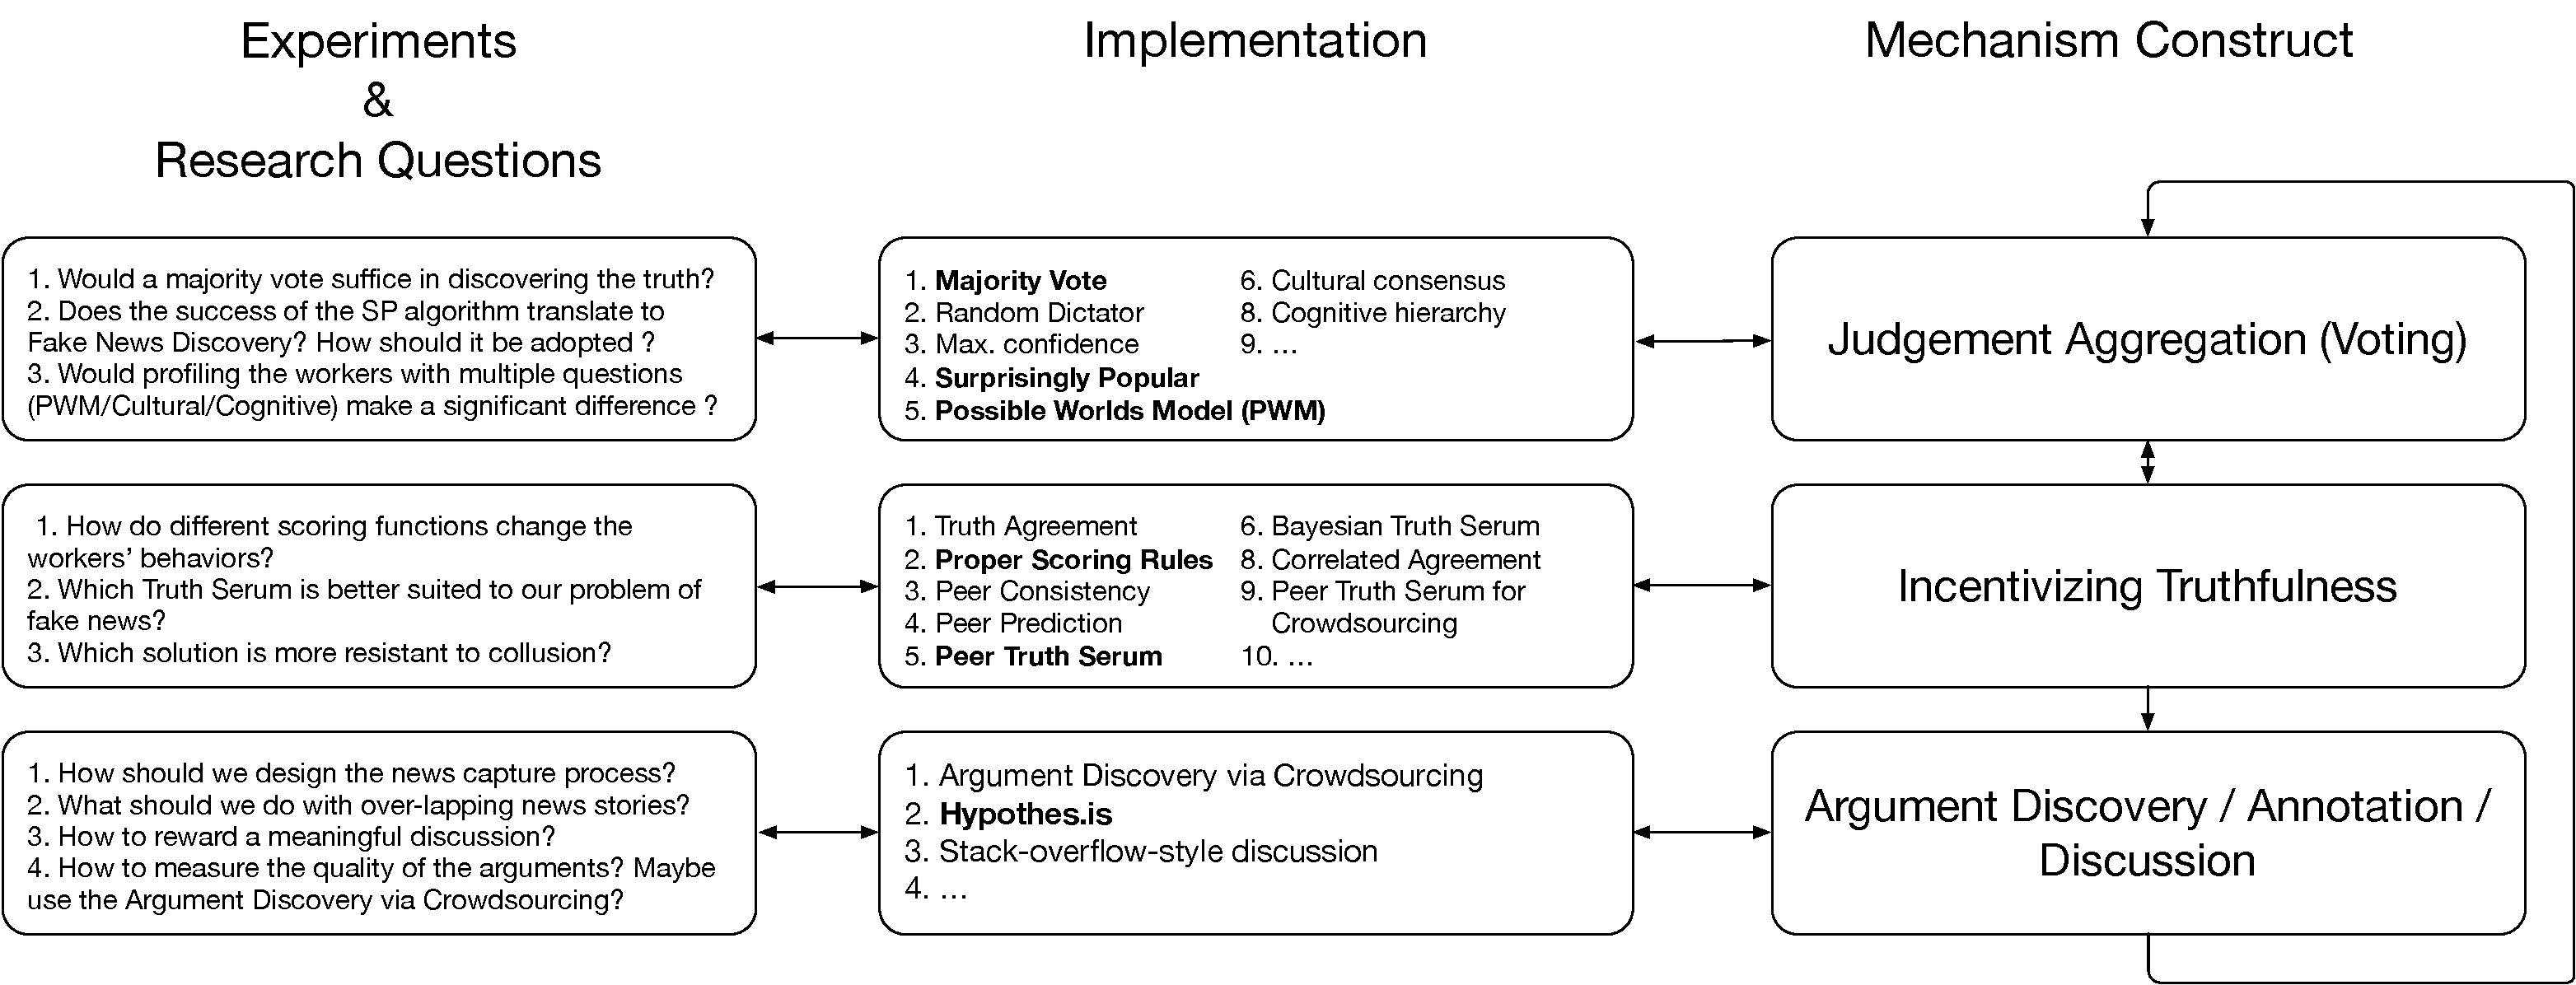
\includegraphics[width=\textwidth]{fake_news_diagram_2.pdf}
    \caption{Overview of the CredibleCrowd mechanism construct, implementation methods and related experiments and research questions}
    \label{fig:overview}
\end{minipage}
\end{figure}

\end{landscape}



\chapter{Judgment Aggregation By Voting}
\label{ch:voting}

\begin{quotation}
    % آنکس که بداند و بخواهد که بداند
    % خود را به بلندای سعادت برساند
    % آنکس که بداند و بداند که بداند
    % اسب شرف از گنبد گردون بجهاند
    % آنکس که بداند و نداند که بداند
    % با کوزه ی آب است ولی تشنه بماند
    % آنکس که نداند و بداند که نداند
    % لنگان خرک خویش به مقصد برساند
    % آنکس که نداند و بخواهد که بداند
    % جان و تن خود را ز جهالت برهاند
    % آنکس که نداند و نداند که نداند
    % در جهل مرکب ابدالدهر بماند
    % آنکس که نداند و نخواهد که بداند
    % حیف است چنین جانوری زنده بماند

    \noindent He who knows not, and knows not that he knows not, shall remain in his double-ignorance till the end of time. He who knows not, and knows that he knows not, shall barely reach his destination. He who knows, and knows not that he knows, shall remain thirsty with water in his pot. \emph{He who knows, and knows that he knows, shall reign over the world.}
\hspace{1em plus 1fill}---Ibn Yamin (Persian Poet)
\end{quotation}



\section{Introduction}
The first phase of CredibleCrowd is truth discovery. In this phase, our focus is on \emph{extracting expertise}. That is, we assume that there are individuals among the population who know the answer. We call them \textbf{experts}; ideally we would find the experts and query their responses. However, since we do not know who the experts are, this is not possible. Nevertheless, our main objective is not to find the expert, but to find the expert opinion. To get the answer we must query the population and aggregate their response via a \emph{voting mechanism}. We start with an important task separation.


\section{Truthful people assumption}
% In authors in \cite{mccoy:stat} and its preceding work \cite{prelec:nature} assume that people are truthful:

\begin{assumption}[Truthfulness]
\label{assum:truthfulness}
``People vote for the world state that they believe is most probable.''
\end{assumption}

 In other words, they believe that eliciting truthful information via modifying the payment function is a separate task . This suggestion is reflected in the separation of Voting and Truthfulness Incentivization phase. In other words the Voting mechanism assumes truthfulness, and leaves the job of ensuring it to the latter phase.
 
 
 \section{Majority Vote}
 A majority vote only uses the actual votes of the respondents. The option with the highest vote is chosen as the outcome of the voting mechanism. However, it is heavily dependent on the majority; in fact, the majority vote is biased for shallow, lowest common denominator information, at the expense of novel or specialized knowledge that is not widely shared.\cite{prelec:nature, chen, lorenz} So the majority vote only extracts the crudest expertise (the \emph{average}) because it collects the the most basic statistics from the respondents.
 



\section{Surprisingly Popular}
In \cite{prelec:nature}, Prelec et al. propose that instead of averaging all the answers, one should give a heavier weight to the experts among the voting population. 

But not knowing who the expert are, how can we do this?
A solution is to ask the respondents about their confidences in their answers, and weight their answers accordingly. We are making two assumptions: that the self-reported confidences are accurate (not over- or under-estimated) and that they correlate well with the correct answer.

Even if those conditions hold (which is unlikely), Prelec proves that no solution based on solicited confidences can give us the correct answer: \cite[Supplementary Information (SI)]{prelec:nature}


\begin{theorem}[Impossibility of first-order knowledge optimality\footnote{The original theorem statement in \cite{prelec:nature} does not include this title. The same for the holds Assumption \ref{assum:bayesian} and Lemma \ref{lemma:2nd_order} that follow.}]
\label{thm:imposibility}
The correct answer cannot be deduced by any algorithm relying exclusively on knowledge of actual signal probabilities, $p(s_k |a_{i^*}), k = 1,\dots ,n$ and posterior probabilities over answers implied by these signals, $p(a_i|s_k), k = 1,\dots, n, i = 1,\dots m$.
\end{theorem}

In the above theorem, $s_k$ is the private \emph{signal} that the respondent receives (which encompasses his knowledge and understanding of the answer) and $a_i$ is the \emph{answer option $i$}. Based on Theorem \ref{thm:imposibility}, we cannot use the confidences to calculate the correct answer. So, what is needed to calculate the correct answer? It turns out that we need to solicit a higher order of knowledge or \emph{Metaknowledge}.

\paragraph{Metaknowledge} is knowledge about knowledge, or \emph{second-order knowledge}. Metaknowledge means that one is aware of what they know or do not know, and of where their level of knowledge stands in relation to other people’s.~\cite{musser:meta} In our problem, metaknowledge translates to the estimations that a respondent makes regarding others answers.

\subsection{World Model}
Prelec uses a particular random variable nomenclature to facilitate his reasoning; but this itself needs some explanation. He assigns a \emph{world} to every answer option. So for a binary question like, ``Do you think this piece of news is real or fake?'' there are two possible worlds. A ``Real'' and a ``Fake'' world. \emph{It is assumed, by construction, that the \emph{correct} answer will be more popular in the correct world than any other world.}


The uncertainty about the answer is thus translated to respondent's uncertainty about the actual world he or she lives in. $a_i$ is the random variable that models this. In our case with two options 'Real' and 'Fake', one observes whether they occupy the Real world or the Fake world; but they do not know the answer to that question with certainty; so they do not know correct world~$a_{i^*}$.

Using the world model jargon, we can state the following assumption about the voters that both authors make~\cite{prelec:nature, mccoy:stat}:

\begin{assumption}[Bayesian Voter]
\label{assum:bayesian}
A respondent is assumed to wish to vote for
the world state that is most likely under their posterior distribution
over world states conditional on their received signal. For the case
of two worlds and two signals this implies that respondents receiving
signal $a$ will wish to vote for world $A$, except in the case where
the signal distribution and world prior is such that world $B$ is
more likely irrespective of the signal received.
\end{assumption}


With this explanation, it is clear that Theorem \ref{thm:imposibility} proves that $p({a_{i^*}} |{ s_k})$, i.e., the (posterior) probability of the correct world given the private signals, cannot be computed using the $p(a_i|s_k), k = 1,\dots, n, i = 1,\dots m$. Prelec instead argues in the following lemma, that the  $p(a_{i^*} | {s_k})$ should be calculated using the estimation of others' private signals (the second-order knowledge):

\begin{lemma}[Role of second-order knowledge]
\label{lemma:2nd_order}
Consider a possible world model with $m$ answers (in our case $m = 2$) and $n$ signals and joint probability distribution $p(s_j, a_i)$. Let $a_{i^*}$ denote the correct answer. Then:

\begin{align}
 p({a_{i^*}} | {s_k}) \propto p({s_k} |{a_{i^*}}) \sum_i\frac{p(s_i|s_k)}{p(s_k|s_i)}
\end{align}


(setting $0/0 \equiv 0$).
\end{lemma}


\subsection{SP voting mechanism}
 Using the Surprising Popular voting mechanism, after gathering the both the votes and predictions of the all the workers, we can see whether True or False has been more popular than expected in either of the worlds. That world is the SP answer. 
 
 \begin{algorithm}[tbh]
    \caption{Surprisingly Popular Voting}
    \label{alg:SP}
    \begin{enumerate}
        \item Agents reports their votes $V^r$
        \item Agents report their predictions of others' responses $M^r\; r=1,\dots, N$ for answer $a_i,\; i=0,1$
        \item Center computes the actual distribution of the votes over the two options $\bar{V}=[v_0, v_1]$
        \item Center computes the mean of predictions M for each answer and forms the mean distribution $\bar{M} = [m_0, m_1]$.
        \item Center calculates the difference vector $\Delta = \bar{V} - \bar{M} = [v_0 - m_0, v_1 - m_1]$
        \item{Center selects $\operatorname{argmax}_{i= 0,1}\delta_i$, where $\Delta = [\delta_0, \delta_1]$}.
    \end{enumerate}
\end{algorithm}

In Algorithm \ref{alg:SP},becuse there are only two options, we have that $\delta_0 = -\delta_1$. Moreover, $|\delta_0|$ is the SP margin of error; the larger it is, the larger the consensus over the SP decision.

% \subsection{Example}
% Imagine a piece of news. The world has a true state $\omega^* \in \Omega$ and  $\Omega = \{A, B\}$. There are two options $\{ \Tilde{A}, \Tilde{B}\}$. $\Tilde{A}$ and $\Tilde{B}$ are opposites: one says that the news is True, while the other says it is False (fake). It is assumed that in state $A$ answer $\Tilde{A}$ is the true answer, while in state $B$, answer $\Tilde{B}$ is correct.

% The correct answer is not known, or equivalently, people do not know what is the true state $\omega^*$ of the world. However, it is assumed that if they knew, they would give a utility of 1 to the true answer and 0 to the other. 

% A worker $w_i$ is given the piece of news and is asked to fact-check it. He uses the sources of information available to him or her, and receives a signal $s \in {a, b}$. 

% Imagine that signal $a$ has probability 0.8
% in state $A$ and probability 0.7 in state $B$ and thus be more likely
% than signal $b$ in both world states. Under this signal distribution,
% if the actual state was $B$ then the majority would receive signal
% $a$, and, assuming a uniform common prior, would vote for state $A$
% and so would be incorrect.

% If the received signal is $a$ assuming that this signal has a uniform common prior, Then, its estimate of the
% probability that the world is in state $A$ is $p(\Omega=A|s=a)=p(s=a|\Omega=A)p(\Omega=A)/p(s=a)=(.8)(.5)/((.8)(.5)+(.7)(.5))$
% and since this quantity is higher than 0.5, workers receiving
% signal $a$ vote that the world is most likely in state $A$. But
% if the actual world is state $B$, workers have a .7 probability
% of receiving signal $a$ and hence the majority of workers will
% vote incorrectly.\cite{mccoy:stat}

\section[Possible Worlds Model]{Possible Worlds Model \protect\footnote{The model in this section is reproduced from \cite{mccoy:stat} with minor changes.}}
\label{sec:PWM}

In the Possible Worlds Model (PWM), McCoy and Prelec build on top the Surprisingly Popular method~\cite{mccoy:stat} by aggregating judgment through a generative framework and Bayesian inference. Figure \ref{fig:pwm_single} illustrates their graphical model for a single question. They assume $N$ respondents who answer binary questions and predict the distribution of the votes by other people --- thus a similar input to the SP. They assume each of the answers ('Real'/ 'Fake') correspond to an underlying world state $\Omega \in {A, B} $ while the actual state of the world $\Omega^*$ is unknown. Respondent $r$ indicates its vote $V^r$ for the answer that he or she believes is most likely, but also makes Meta-predictions $M^r$. Moreover, the respondent $r$ receives a private signal $T^r$ and observes the public prior on the signal distribution $S$ which is a $2 \times 2$ left-stochastic (columns sum to 1) matrix for binary classification. Element $S_{i,j}$ is the probability of receiving signal $i$ when the true world state $\Omega^* = j$.

Importantly, McCoy and Prelec do not assume that if $\Omega^* = i$ then signal $i$ is necessarily the most probable signal. Instead they assume that the $S$ is sampled uniformly from the set of left stochastic matrices with the constraint that $ p(T^r = i| \Omega = i) > p(T^r = i| \Omega = j), \; i, j \neq i $.

Noise in voting data is allowed by making a respondent’s vote a softmax decision function of the posterior distribution, with the voting noise parameter $N_V$ giving the temperature of this function. The voting noise parameter is drawn from a \texttt{Gamma(3, 3)} distribution.

\subsection{Making a voting decision}

A respondent
$r$ receiving signal $k$ has all the information necessary to compute
a posterior distribution: 
\begin{align}
p(\Omega=j|T^{r}=k,S,\Psi)=p(T^{r}=k|\Omega=j,S)p(\Omega=j|\Psi)/p(T^{r}=k)
\end{align}
over the world states. Knowing the posteriors, the respondent can vote under the following assumption:



\subsection{Metaknowledge: Predicting other voters}
A respondent $r$ who received signal $k$
has the information required to compute the posterior distribution
$p(T^{s}=j|T^{r}=k)$ over the signals received by an arbitrary respondent
$s$: 
\begin{align}
    p(T^{s}=j|T^{r}=k)=\sum_{i}p(T^{s}=j|\Omega=i)p(\Omega=i|T^{r}=k)
\end{align}
and marginalizing over possible worlds.

\subsection{Extension to multiple questions}
Figure \ref{fig:pwm_multiple} shows the extension of PWM to multiple questions. The multiple-question model is very similar to the single-question one. The main addition is the incorporation of respondent's expertise across $Q$ different questions. It is important to note that questions are more or less independent: the world prior, (actual) world, signal distribution and noise parameters are sampled per question. Authors model the \emph{expertise} of respondents  by how likely they are to receive the correct signal, this is called the 'information expertise' and shown as $I^r$ in the graphical model in Figure \ref{fig:pwm_multiple}.

\subsection{Miscellaneous schemes}
While in this chapter, we mainly focused on the Surprisingly Popular and Possible World Model, we should mention other voting schemes that do not require as much analysis. For example, in the \textbf{Random Dictator} voting scheme, we choose at random  one of the voters and accept his vote as the correct~answer. 

We conclude by mentioning two other generative models (similar to PWM). The \textbf{Cultural Consensus} model is used to extract \emph{cultural knowledge}. Respondent answers are used to determine the extent to which each individual knows the culturally correct answers (their ‘cultural competence’) and the cultural consensus is then determined by aggregating responses across individuals with the answers of culturally competent people weighted more heavily. The \textbf{Cognitive Hierarchy} model captures the `expertise' or 'knowledge level' of respondents via latent variables, in which all respondents have to answer a set of questions.



\newpage
\thispagestyle{empty}
\begin{figure}[]
 \vspace*{-3cm}
\begin{subfigure}{\textwidth}
    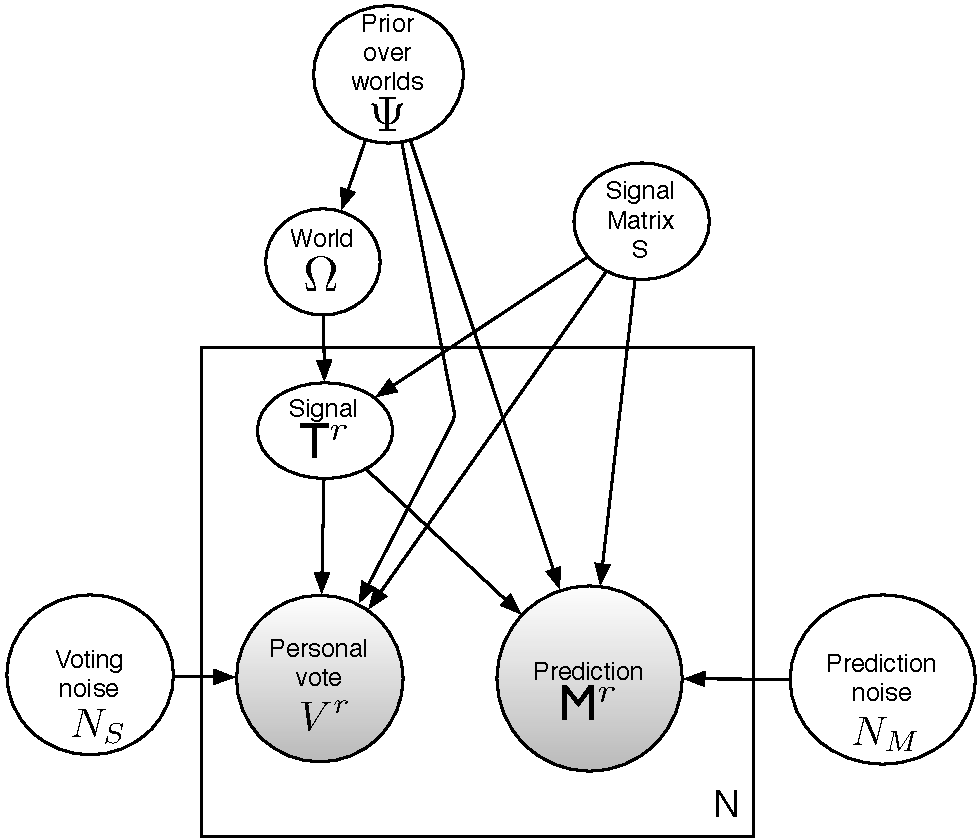
\includegraphics[width=\textwidth]{basic_generative_votes_updated.pdf}
    \caption{The single question possible worlds model which is used to infer the underlying world state based on a group’s votes and predictions of the votes of others.}
    \label{fig:pwm_single}
\end{subfigure} \\
\begin{subfigure}{\textwidth}
    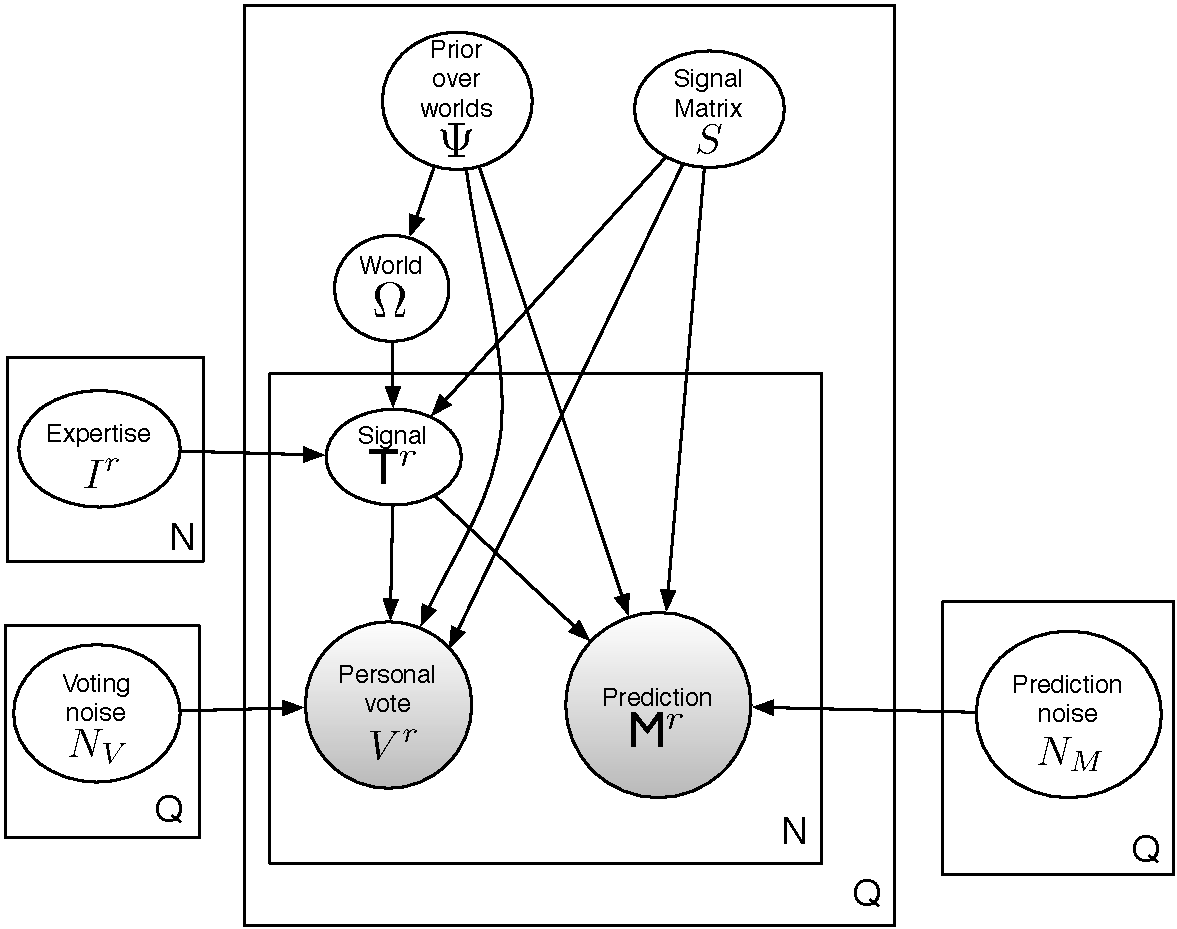
\includegraphics[width=\textwidth]{generative_individual_expertise_votes_updated.pdf}
\caption{The multiple question Possible World Model which is applied across questions for N respondents answering Q questions.}
\label{fig:pwm_multiple}
\end{subfigure}
\caption{[From reproduced from \cite{mccoy:stat}] The Possible Words Model (PWM). In standard graphical model plate notation nodes are random variables, shaded nodes are observed, an arrow from node X to node Y denotes that Y is conditionally dependent on X, a rectangle around variables indicates that the variables are repeated as many times as indicated in the lower right corner of the rectangle.}
\end{figure}

% \begin{figure}[H]
%     \centering
%     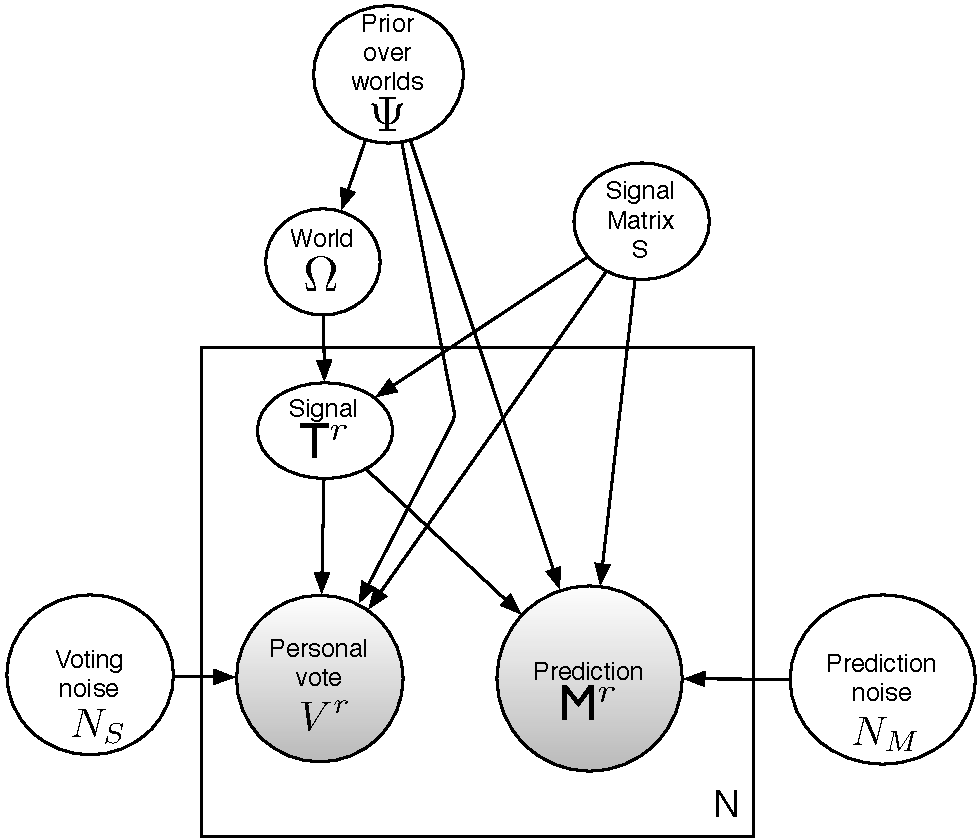
\includegraphics[width=\textwidth]{basic_generative_votes_updated.pdf}
%     \caption{The single question possible worlds model (PWM) which is used to infer the underlying world state based on a group’s votes and predictions of the votes of others. In keeping with standard graphical model plate notation, nodes are random variables, shaded nodes are observed, an arrow from node X to node Y denotes that Y is conditionally dependent on X, a rectangle around variables indicates that the variables are repeated as many times as indicated in the lower right corner of the rectangle.}
%     \label{fig:pwmsingle}
% \end{figure}

% \
%     \centering
%     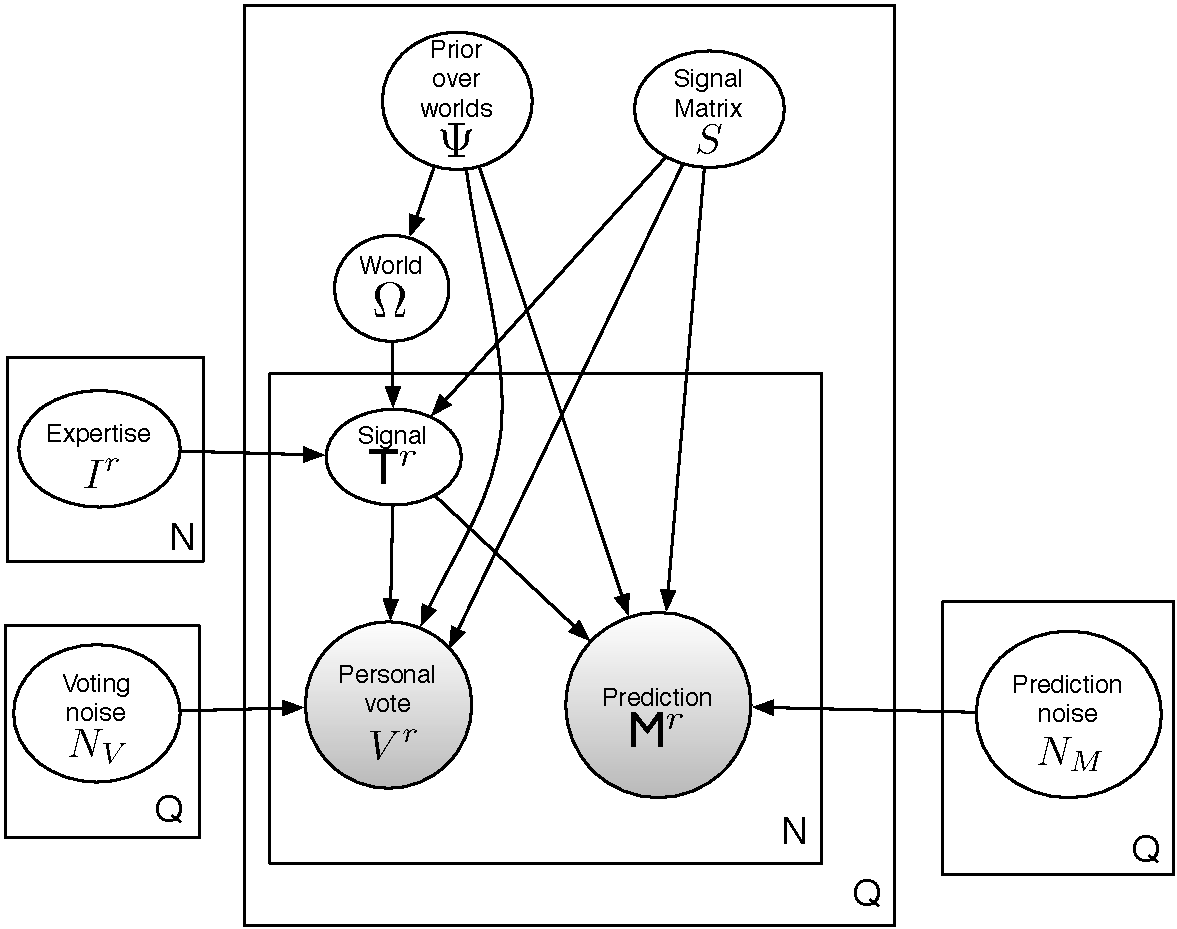
\includegraphics[width=\textwidth]{generative_individual_expertise_votes_updated.pdf}
%     % \caption{The single question possible worlds model (PWM) which is used to infer the underlying world state based on a group’s votes and predictions of the votes of others. In keeping with standard graphical model plate notation, nodes are random variables, shaded nodes are observed, an arrow from node X to node Y denotes that Y is conditionally dependent on X, a rectangle around variables indicates that the variables are repeated as many times as indicated in the lower right corner of the rectangle.}
%     % \label{fig:pwmsingle}
% \end{figure}





\chapter{Eliciting Truthful Information}
\label{ch:truthful}
\section{Introduction}
In the previous chapter, we started with the assumption that, as far as the voting mechanism is concerned, respondents are truthful, in the sense that 1) they make an effort to learn the answer and 2) they vote according to their updated beliefs. In Chapter \ref{ch:overview} we called this the \textbf{Truthful behavior}, and contrasted the \emph{truth-seeking} individuals with those who are \emph{reward-seeking}.

In this section, we revoke that assumption and design reward (payment) schemes that incentivizes individuals to vote and report truthfully. Throughout this chapter we assume that voters are reward-seeking individuals and that they consider only the monetary value of the reward, and not the outcome of the mechanism (i.e., compensation is not in influence over the outcome of the mechanism). Table \ref{tab:tax} summarizes the nomenclature we will be using in this chapter.

In this chapter we summarize the theoretical concepts we need to design the second phase of the CredibleCrowd system. What follows is in essence a short excerpt of the necessary tools and concepts in~\cite{faltings:book}.

% \begin{itemize}
% \nitem[Center (Us)] Who collects the data from workers
% \nitem[Data] 
% \begin{itemize}
%     \nitem[Objective] every agent observes the same realization of the phenomenon.
%     \nitem[Subjective] each agent observes a possibly different realization of the same phenomenon.
% \end{itemize}
% \nitem[Center Goals]
% \begin{itemize}
%     \item Objective Data => Most Accurate Data
%     \item Subjective Data => Obtain distribution of values observed by agents. 
% \end{itemize}

% \nitem[Verifiability]
% \begin{itemize}
%     \nitem[Verifiable] Center will eventually get access to the ground truth.
%     \nitem[Unverifiable] There is no Ground Truth.
% \end{itemize}
 
%  \item (Worker) Strategies
%  \begin{itemize}
%      \nitem[Heuristic] reported value does not depend on an observation of the phenomenon.
%      \nitem[Cooperative] the agent invests effort to observe the phenomenon and truthfully reports the observation.
%  \end{itemize}
 
%  \item Truthful Strategies
%  \begin{itemize}
%      \item Agents report their belief about the phenomenon truthfully.
%      \item $\text{Cooperative} \subset \text{Truthful}$
%  \end{itemize}
%  \end{itemize}
 
 
\begin{table}[]
\centering
\small
\caption{Nomenclature and Taxonomy}
\label{tab:tax}
\begin{tabular}{@{}lll@{}}
\toprule
Term            & Subcategory & Definition                                                                                                                                  \\ \midrule
Agent           & Center      & Data Collector (or Requester)                                                                                                               \\[1mm]
                & Worker      & Crowd-sourcing agent                                                                                                                        \\ \midrule
Data            & Objective   & \begin{tabular}[t]{@{}l@{}}Every agent observes the same realization \\of the phenomenon.\end{tabular}                                     \\[4mm]
                & Subjective  & \begin{tabular}[t]{@{}l@{}}Each agent observes a possibly different \\realization of the same phenomenon.\end{tabular}\\[4mm]
                & Verifiable  & There (eventually) is a ground truth.                                                                                                       \\[1mm]
                & Unverifiable  & No ground truth                                                                                                                             \\ \midrule
\begin{tabular}[t]{@{}l@{}} Worker\\Strategy\end{tabular} & Heuristic & \begin{tabular}[t]{@{}l@{}}Agent slacks and the reported value \\does not depend on an observation.\end{tabular}                              \\
                & Cooperative & \begin{tabular}[t]{@{}l@{}}Agent invests effort to observe the  phenomenon\\ and truthfully reports the observation.\end{tabular}           \\
                & Truthful    & \begin{tabular}[t]{@{}l@{}}Agents report their belief about the\\ phenomenon truthfully. (Truthful $\subset$ Cooperative)\end{tabular} \\ \midrule
Compensation    & Monetary    & Actual money, reputation points, rewards, etc. \\
                & Influence   & \begin{tabular}[t]{@{}l@{}}leverage on the model that the center learns \\from data. \end{tabular}\\\bottomrule
\end{tabular}
\end{table}
 
%  \subsubsection{Types of data/tasks}
%  \begin{itemize}
%      \nitem[Objective Data] each task (news piece) has a state (True/False) that each worker observes and reports. \textit{Or} 
%      \nitem[Subjective Data] each worker has a different belief about the veracity of a given task, and we want to correctly poll these opinions.
%  \end{itemize}


\subsection{What to strive for in a mechanism?}
\paragraph{Truthfulness} induces agents to choose a cooperative and truthful strategy.
\paragraph{Individually Rational} where agents can expect a positive utility from participating.
\paragraph{Positive Self-selection} which means only agents that are capable of providing useful data can expect a positive utility from participating.




\subsection{Belief: The agent's local information}
Our mechanisms use agents' self-interest to influence their strategies. This influence depends crucially on how observations influence the agent’s beliefs about the phenomenon and about the reward it may receive for different strategies. The belief of an information agent is characterized by a prior probability distribution 
\begin{equation}
    P_i(x) = {p_i(x_1), ..., p_i(x_n)}
\end{equation}
of what the state X of the phenomenon might be.

Following an observation, based on the received signal $s_i$ it will update its prior belief
\begin{equation}
    P_i(X=x | S_i = s) = P_i(x|s)
\end{equation}
to a posterior distribution, thus a new belief. It is assumed that the new belief contains all the information observed from the signal.

\subsubsection{Belief Update}
Belief update is done using the Bayes Law. When the probability distribution is given by the relative frequencies of the different values, the update could be weighted mean between the new observation and the prior distribution:

\begin{equation}
\label{eq:linear_belief_update}
    \hat{q} = \begin{cases} 
(1-\delta)p(x) + \delta &\text{for } x=o \\
(1 - \delta)p(x)        &\text{for } x\neq o 
\end{cases} = (1 - \delta)p(x) + \delta.\mathbbm{1}_{x=o}
\end{equation}

$\delta$ is a parameter that can take different values according to the weight that that an agent gives to its own measurement vs. that of others. We will call $\delta$ the \textbf{learning rate} from hereon. 

Two important properties of the belief update is \textbf{self-dominating} for objective data and (an easier condition to satisfy) \textbf{self-predicting} for subjective data.

\begin{definition} An agent's belief update is self-dominating if and only if the observed $o$ has the highest probability among all possible values $x$:

\begin{equation}
    q(o|o) > q(x|o), \forall x \neq o.
\end{equation}
\end{definition}
\begin{example}
$\delta = 1/t$ would compute the moving average if $o$ is the $t$'th observation.
\end{example}

\begin{definition}
\label{def:self_predicitng}
An agent's belief update is self-predicting if and only if the observed $o$ has the highest relative increase in probability among  among all possible values:

\begin{equation}
    q(o|o)/p(o) > q(x|o)/p(x), \forall x \neq o.
\end{equation}
\end{definition}






See Table \ref{tab:summary} for a summary of the relation between verifiability, objectivity and ground truth.

\begin{table}[]
\centering
\caption{Verifiability $\Longleftrightarrow$ Objectivity $\Longleftrightarrow$ Ground Truth}
\label{tab:summary}
\footnotesize
\begin{tabular}{@{}llll@{}}
\toprule
Verifiability & Objectivity             & Ground Truth                                                                                                                                                                             & Example                                                             \\ \midrule
Verifiable    & Objective               & Always exists for the true value                                                                                                                                                         & \begin{tabular}[t]{@{}l@{}}Temperature \\ Measurements\end{tabular} \\
Unverifiable  & \begin{tabular}[t]{@{}l@{}}Objective\\ \\
Subjective\\\end{tabular} & \begin{tabular}[t]{@{}l@{}}Doesn't exist for \\individual data (worker reports).\\ Exists for distribution of the reports \\(Every worker samples from\\ the same distribution.)\end{tabular} &\begin{tabular}[t]{@{}l@{}}\\ Restaurant\\ Reviews \end{tabular}                                                
\end{tabular}
\end{table}

\section{Mechanisms for verifiable information}

Two simple mechanisms for verifiable information is Truth Agreement for objective data and Proper Scoring for subjective data.

\subsection{Truth Agreement}
This is a simple mechanism for objective data. We pay the worker (the respondent) only if his answer matches (the later discovered) ground truth.

\begin{algorithm}
    \caption{Truth Agreement}
    \label{alg:truth_agreement}
    \begin{enumerate}
        \item Agent reports data = (discrete) value x.
        \item Center observes the ground truth g (at some later time).
        
        \item{Center pays agent a reward:
        \begin{equation*}
            pay(x, g)=
            \begin{cases}
                 1 &\text{ if x = g}\\
                 0 &\text{ o.w.}
            \end{cases}.
        \end{equation*}}
    \end{enumerate}
\end{algorithm}

Although this is a very simple mechanism, it is very popular for crowd-sourced data labeling. This is done by scoring workers' performance via their answers to the \emph{gold tasks}, for whcih we know the ground truth, and rewarding the workers only by those answers.

\subsection{Eliciting Distributions: Proper Scoring Rules}
\label{sec:proper}

\begin{algorithm}[b]
    \caption{Scoring Rule}
    \label{alg:scoring_rule}
    \begin{enumerate}
        \item Agent reports data = probability distribution A.
        \item Center observes the ground truth g (at some later time).
        
        \item{Center pays agent a reward:
        \begin{equation*}
            pay(A, g)= SR(A, g),
        \end{equation*}}
        where $SR$ is a \emph{proper scoring} rule.
    \end{enumerate}
\end{algorithm}

\subsubsection{Proper Scoring rule}
Since we are asking workers to provide a probability vector (a distribution), we need a scoring function to calculate worker's reward. A \emph{proper} scoring function is one that gives the highest expected reward if the worker reports the true probability distribution that he or she observes; thus reducing the incentive for dishonesty. The \textbf{Quadratic} scoring rule is an example of an strictly proper:
\begin{equation}
    Q(A, g) = 2a_g - \sum^C_{j=1} {r_j^2}, 
\end{equation}
where $a_g$ are probabilities reported for each class of the outcome and $C$ is the number of classes. The \textbf{Brier} scoring rule is calculated based on the Quadratic rule as follows:
\begin{equation}
    B(A, g) = \sum_{j=1}^C (y_j -r_j)^2.
\end{equation}

\section{Parametric mechanisms for unverifiable information}

\paragraph{Leveraging peer consistency}
To validate data, we need to use its coherence with data submitted by the agents who observe the same phenomenon.

\subsection{Peer consistency for objective information}
The idea is simple: an agent will only be paid if her answer matches that of a randomly selected peer.

\begin{algorithm}
    \caption{The output agreement mechanism.}
    \label{alg:output_agreement}
    \begin{enumerate}
        \item Center gives a task to agents $a_i$; $a_i$ reports data $x_i$.
        \item Center randomly selects a peer agent $a_j$ that has also been given the same task and reported data $x_j$.
        
        \item{Center pays agent $a_i$ a reward:
        \begin{equation*}
            pay(x_i, x_j)= \begin{cases}
                 1 &\text{ if } x_i = x_j\\
                 0 &\text{ o.w.}
            \end{cases}.
        \end{equation*}}
    \end{enumerate}
\end{algorithm}



\subsection{Peer consistency for subjective information}
There are two (separate) sets assumptions for designing peer consistent mechanisms for subjective information:
\begin{enumerate}
    \item A homogeneous agent population with \emph{identical and known prior and posterior beliefs}. Ex. Peer Prediction
    
    \item Common and known prior beliefs, but \emph{belief updates can be heterogeneous} as long as they satisfy the self-predicting condition
    Ex. Peer Truth Serum (PTS).
\end{enumerate}

We will start with peer prediction, state the algorithm, discuss its limitations and proposed remedies; and finally motivate the peer truth serum.


\subsection{Peer prediction}
\begin{algorithm}[H]
    \caption{Peer Prediction}
    \label{alg:peer_prediction}
    \begin{enumerate}
        \item Center gives a task to agents $a_i$; $a_i$ reports data $x_i$.
        \item Center randomly selects a peer agent $a_j$ that has also been given the same task and reported data $x_j$.
        
        \item Center selects an assumed posterior distribution $\hat{q}_{x_i}$ associated with report $x_i$.
        
        \item{Center pays agent $a_i$ a reward:
        \begin{equation*}
            pay(x_i, x_j)= SR(\hat{q}_{x_i}, x_j),
        \end{equation*}}
        where $SR$ is a \emph{proper scoring} rule.
    \end{enumerate}
\end{algorithm}

Reward calculation is done using a proper scoring function, as follows:

\begin{enumerate}
   \item Each value for answer $x_i$ is associated with an assumed posterior distribution $\hat{q}(x) = \hat{\Pr}(x|x_i)$.

 \item $\hat{q}$ is skewed so that $x_i$ is more likely than in the prior.

 \item A proper scoring rule is used to score this posterior against a random peer report.
\end{enumerate}



\subsection{Peer Prediction Problems}
The Peer Prediction (Algorithm \ref{alg:peer_prediction}) payments illustrate two problems that are not unique to this approach:

\begin{enumerate}
    \item General proper scoring rules generate \textbf{inefficient} and \textbf{volatile payments}: the center has to potentially pay a huge premium to elicit truthfulness.

    \item Mechanism can have other, more profitable but \textbf{uninformative equilibria}, i.e., always reporting the same answer.
    It is possible to show that any mechanism based on just 2 reports will always have uninformative equilibria with a higher payoff than the truthful one.

\end{enumerate}

 \emph{Automatic mechanism design} can alleviate both problems: 
 
 \begin{enumerate}
     \item It solve an optimization problem to minimize the expected payments by adjusting the rewards.
     \item Constrain the optimizer on the distribution of multiple peer reports to avoid uninformative equilibria.
 \end{enumerate}

However, there are more conceptual problems with peer prediction:

\begin{itemize}
 \item Mechanism designer should know the exact posterior distributions formed by an agent for each different observation.
 
 \item Moreover, these distributions have to be the same for every agent that participates in the mechanism!
\end{itemize}

This problem can be alleviated using a technique called \textbf{shadowing} which we will explain by means of an example:

\paragraph{Shadowing} Imagine a scenario where agents have to submit good or bad reviews for a restaurant review. Imagine the quality `bad' was observed, $o = \text{`bad'}$. For truthfulness guarantee, we must have that when agent increases posterior probability $q(`bad')$ over the prior when observing `bad' it happens that the expected reward 
\begin{equation}
    \mathds{E}[pay(\text{`bad'}) | o = \text{`bad'}] > 
    \mathds{E}[pay(\text{`good'}) | o = \text{`bad'}],
\end{equation}
for any $\delta$ that satisfies some well-formedness constraints of the distribution~\cite{faltings:book}. Therefore the exact value of the $\delta$ does not matter. 

\subsection{Spurious signals in peer prediction}

The trick is that the common signal that allows the agents to coordinate their strategies is the phenomenon they can all observe.\cite{faltings:book} However, the true signal (the phenomenon which a piece of news describes) should be the only coordinating signal among two workers. Ensuring that the peers would not coordinate on some other signal is difficult. Indeed, it is due to these spurious signals that some uninformative equilibria are formed:

\subsubsection{Why Peer prediction wouldn't work as expected}

``The main idea behind peer-prediction mechanisms can be understood as a `clever majority vote'—every agent is paid according to a specific similarity between her and her peer. For example in the case of peer-grading in a class, coordinating on just checking the grammar can guarantee good agreement with other agents, but with substantially reduced effort.''~\cite{kong:noverify}
    
Gao et al point out that things are likely even worse than this. ``If the cheap signals correlate more than the expensive signals, then the peer-prediction techniques incentivize agents to not report the true answer, but instead focus on cheap signals! For example, in the essay grading above, it is likely that assessments of grammatical correctness will agree more than assessments of overall essay quality. Because of this, peer-prediction mechanisms will pay agents more overall for lower-quality information.''~\cite{kong:noverify} So there is a clear incentive for collusion. 
    
One approach to counter coordinated low-quality strategies is to use trusted agents that provide the correct answers for some randomly selected subset of tasks. In a hybrid mechanism, agents’ reports will be either compared to other agents, or to such trusted reports. If the probability of having a trusted agents as a peer is sufficiently high, other low-quality equilibria can be broken. However, it has recently been shown that if the coordinated low-quality strategy provides higher payoffs than the cooperative strategy (for example, because it involves no measurement noise), it may be better to use simple truth agreement rather than a combination with peer consistency mechanisms as a complement to the truthful reports.~\cite{boi:book, gao:peer}






\section{Peer Truth Serum}
\label{sec:peer_truth_serum}
The construction of the posterior can be bypass altogether by using the Peer Truth Serum from Prelec et al. (See Section \ref{sec:peer_truth_serum}).

\begin{algorithm}[H]
    \caption{The peer truth serum (PTS)}
    \label{alg:peer_truth_serum}
    \begin{enumerate}
        \item Center informs all agents of prior distribution $R$ used by the mechanism.
        \item Agents $a_i$ carries out a task and observes value $o$; $a_i$ reports data $x_i$ .
        
        \item Center randomly selects a peer agent $a_j$ that has also been given the same task and reported data $x_j$.
        
        \item{Center pays agent $a_i$ a reward:
        \begin{equation*}
            pay(x_i, x_j)= \frac{\mathbbm{1}_{x_i = x_p}}{r(x_i) -1},
        \end{equation*}}
        where $r(x_i)$ is the frequency of the answer $x_i$. 
    \end{enumerate}
\end{algorithm}

The derivation of the reward is based on using a logarithmic scoring rule and the linear belief update we saw in Equation \ref{eq:linear_belief_update}~\cite[p42]{faltings:book}. The payment rule by construction aligns incentives between the reporting agents and the model learning process of the center.

\subsection{Peer Truth Serum: Pros}
The peer truth serum enjoys important properties. First, it can be proved that if the belief updates are self-predicting (see Definition \ref{def:self_predicitng}) then there exists a strict ex-post subjective Bayes-Nash equilibrium where all agents are reporting truthfully. This result basically means that the mechanism is strategy-proof; meaning that no agent (worker) can increase his or her payoff by reporting an untruthfully. In fact, the payoff will be strictly smaller than the truthful strategy.

Moreover, it is shown that the self-predicting condition is a condition that cannot be so easily relaxed, and therefore the mechanism is essentially unique.~\cite{faltings:book}

Another good feature of the Peer Truth Serum is that its expected pay increases linearly with agent's confidence, so PTS incentivizes agents to invest more effort to increase their confidence in their reported data.

\subsection{Peer Truth Serum: Cons}
PTS does not solve the problem of unhelpful equilibria. The reason is that PTS still depends on the common prior $R$, that it has to publish to all agents. Agents have to coordinate on this prior. However, there is no guarantee that they would not also coordinate on some other spurious signal.

The second problem is shared by all of the mechanisms we studied. All mechanisms depend on belief updates to incentivize truthfulness. However, most of the mechanisms we studied thus far take beliefs as \textbf{parameters} input to the system. Parameters are undesirable because 1) they are very hard to guess for the Center, and 2) since mechanisms are designed for the whole population of the agents, the parameters have to be very uniform.

To do away with the priors, we need to replace them with new statistics. We can either elicit beliefs directly from workers (which motivates the Bayesian Truth Serum), or learn the distributions through observing agents' reports (Peer Truth Serum for Crowdsourcing).

\section{Bayesian Truth Serum (BTS)}
This is the counter part of the Surprisingly Popular voting scheme that we saw in Chapter \ref{ch:voting}. In BTS, we ask the agents to provide both the data of interest, as well as prediction reports which are agents' predictions on what other agents report as data, i.e.,  the agent’s posterior belief $q$ about the data:

\begin{algorithm}
    \caption{The original Bayesian truth serum (BTS)}
    \label{alg:bayesian_truth_serum}
    \begin{enumerate}
        \item{Center gives the same task to agents $A = \{a_1,\dots,a_k\}$. Each agent $a_i$ reports an \emph{information report} $x_i$ and a \emph{prediction report} $F_i$, where the prediction report is an estimate of the distribution of answers $x_i$ among agents in $A$.}
        
        \item{To compute the score of agent $a_i$, the center computes the histogram of information reports $\operatorname{freq}_{-i}(x)$ and the geometric mean of prediction reports $\operatorname{gm}_{-i}(F)$, where $-i$ means that the reports of $a_i$ are excluded from the mean.}
        \item{The center computes the prediction score 
       
        \begin{equation*}
            \tau_{pred} = -\operatorname{D}_{KL}(freq_{-i}(x)|| F_i(x))(x),
        \end{equation*} 
        and the information score
        \begin{equation*}
        \tau_{inf} = \ln{\operatorname{freq}_{-i}(x_i)} - \ln{\operatorname{gm}_{-i}(x_i)}.
        \end{equation*}}
        \item{The center rewards $a_i$ with a payment proportional to:
            \begin{equation*}
                \tau_{BTS}(x_i, F_i) = \tau_{inf} + \tau_{pred}
            \end{equation*}}
    \end{enumerate}
\end{algorithm}

The BTS comes in several versions. There is a robust version that can work with a small number of reports. The divergence-based version alleviates the need for a large number of agents or self-predicting constraints. However, BTS has had limited success in practice.~\cite{faltings:book}

\section{Miscellaneous mechanisms}
There are a class of mechanisms that use multiple reports to build the second-order statistics necessary for the payment scheme. These are the \textbf{Correlated Agreement}~\cite{dasgupta:correlated} and the newly introduced \textbf{Peer Truth Serum for Crowdsourcing}. The first makes use of the correlation between the answers given to multiple questions by multiple randomly selected agents who have reported answers to the same questions, while PTS for Crowdsourcing uses the histogram of the values received for a particular question, and rewards the \emph{surprisingly common} answers. Common because they match those of a peer, and surprising because less likely answers carry a higher reward.~\cite{radanovic:PTS-CS}
 
\chapter{Experiments and Results}
\label{ch:experiments}
Since we are dealing with judgments from real people, we must base our mechanisms on observations from real crowds. Therefore, we design and conduct experiments to gauge the performance of different models at each phase of the system.

The current work only deals with the first phase, ``Judgment Aggregation.'' Nevertheless, in the future work's section, we outline the design and requirements of  experiments for second and third phases.

\section{Experiment 1}
In this experiment, we want to answer these research questions:

\begin{enumerate}
    \item Would a majority vote suffice in discovering the truth?
    \item Does the success of the SP algorithm translate to Fake News Discovery? How should it be adopted ?
\end{enumerate}

For this first experiment, we used the crowd-sourcing platform, Amazon Mechanical Turk (AMT). In AMT, a \textbf{requester} can post Human Intelligence Tasks (\textbf{HITs}) on a ledger, and MTurk \textbf{workers} with (optional) qualifications can accept the HIT and start working on this.

AMT is frequently used for tasks that are still onerous for machines to perform well, including labeling datasets etc. However, many researchers in varied fields from Human Cognition and Neuroscience to Psychology and Behavioral Studies, have been using AMT as a platform to perform controlled-experiments. In fact, these have become so frequent that toolchains have been created to ease the process of conducting such experiments like \emph{psiTurk}.

\subsection{Experiment Setting}
In the standard AMT fashion, separate HITs need to be created for each and every question. However, to avoid an unbalanced dataset of answers, we designed a single web-page HIT for this experiment where we asked our respondents to answer three questions about each of the 11 news pieces that we have selected from a labeled dataset of fake news~\cite{allcott:stanford}:

\begin{enumerate}
    \item Is this news piece real or fake?
    \item How confident are you in your answer?
    \item What percentage of other American Mechanical Turk respondents do you think would answer "Real" to the first question?
\end{enumerate}

The experiment was designed to replicate ``Study 1c -- State capitals'' in \cite{prelec:nature}. The respondents had to provide a percentage above 50\% for question 2, and a percentage between 0 and 100\% for question 3. Moreover, in order to ensure that respondents have read the article, and are not just filling out the form randomly, we ask a forth question about a \emph{honeypot} embedded in the text.

\paragraph{Honeypot} is a relatively easy riddle to be solved by respondents for validating their engaged (effortful) answers before continuing to the next question. It is embedded into the news text, as an out-of-context sentence about a semantically unrelated thing like a fruit. Honeypots are hard to recognize by a syntax- or style-minded parser, but are obvious to a semantic-minded one.

\paragraph{Remuneration} To replicate the experiment carried out by Prelec et. al in \cite{prelec:nature}, we decided to use an almost identical remuneration scheme to theirs. Therefore, the participants were paid a flat participation fee of \$2 for their participation in the 10-minute study regardless of their answers. 

\paragraph{Bonuses} To incentivize effortful work, two  bonuses were devised. The first bonus was calculated based on the accuracy of the respondent and his or her expressed confidence. The scores in table of Figure \ref{fig:first_page} are calculated using the Brier scoring function (see Section \ref{sec:proper}). The bonus went to the top 20\% with the highest scores. The second bonus was calculated based on the accuracy of the crowd estimations and went to the top 20\% participants with the best estimations.

\begin{figure}[H]
    \centering
    \vspace*{-2cm}
    \makebox[\linewidth]{
    
\includegraphics[width=1.5\textwidth]{experiement_sample_question.pdf}
    }
    \caption{Sample question from Experiment 1}
    \label{fig:sample_question}
\end{figure}


\newpage
\thispagestyle{empty}
\begin{figure}[H]
    \centering
    \vspace*{-4.2cm}
    \makebox[\linewidth]{
    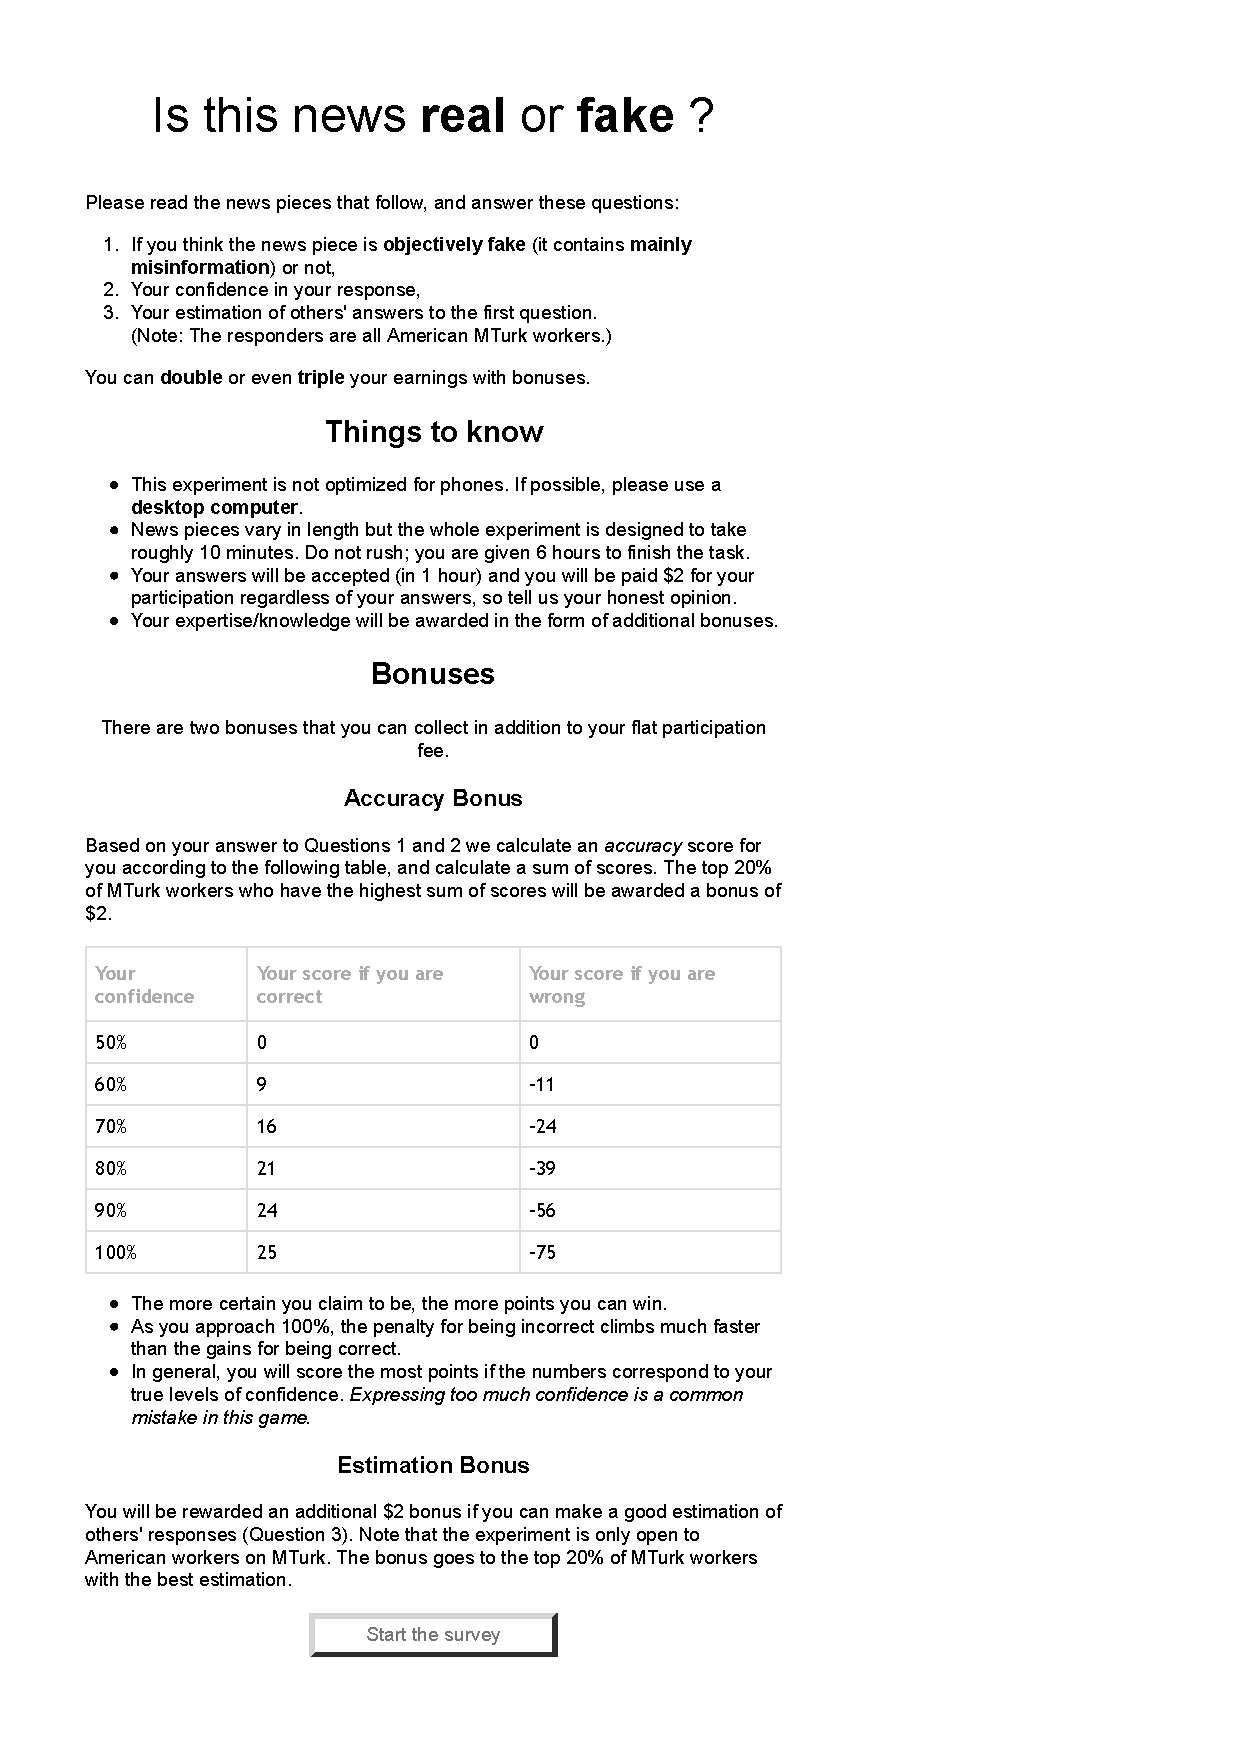
\includegraphics[trim={0 0cm 0 0cm}, clip, width=1.1\textwidth]{true_fake_first_page.pdf}
    }
    \caption{Instructions Page for Experiment 1}
    \label{fig:first_page}
\end{figure}



\subsection{Results}
50 participants took part in the experiment. 3 of the respondents submitted the experiment prematurely and as such their data was removed from the dataset.

\subsection{Accuracy}
The experiment contained 7 fake news articles and 4 real ones. Respondent's are not accurate on average (Figure \ref{fig:exp1_acc}). The majority of answers are in fact, incorrect. Less than 25\% of the respondents give accurate answers (more than 70\% accuracy) and almost than 50\% give fairly inaccurate answers (less than 50\% accuracy).

\begin{figure}
    \vspace*{-1cm}
    \centering
    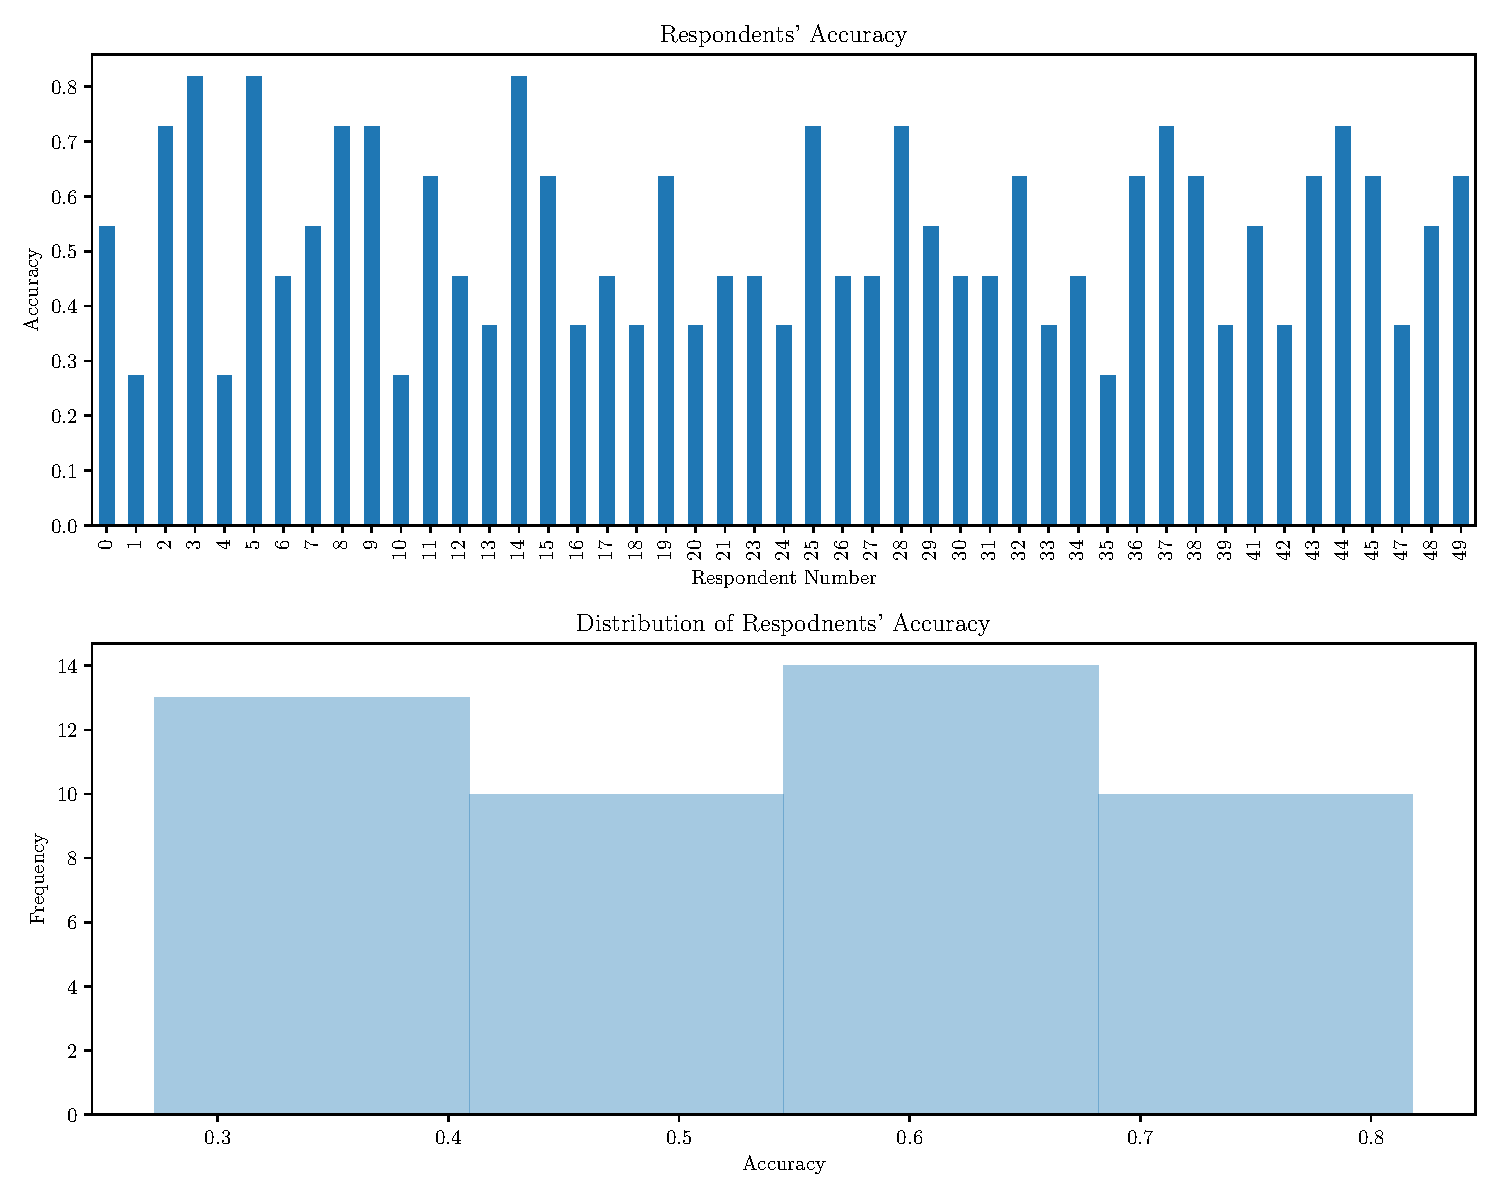
\includegraphics[width=\textwidth]{exp1_accuracy.pdf}
    \caption{AMT Respondents are not very accurate. The mean accuracy is only 53\%.}
    \label{fig:exp1_acc}
\end{figure}

\subsection{Confidence}
\label{sec:conf}
Figure \ref{fig:conf_hist} shows the histogram of confidences expressed by respondents in each trial. We observe a wide range of confidences in most trials. For most of the trials, the reported confidence seems very uninformative. Indeed, as we see in section \ref{sec:baseline_comparison}, weighting the majority vote with the confidences expressed makes little difference in the performance of the majority vote.

\newpage
\begin{center}
\hspace*{-3cm}
\begin{minipage}{1.5\linewidth}
\begin{figure}[H]
\captionsetup{singlelinecheck = false, justification=justified}
    \centering
    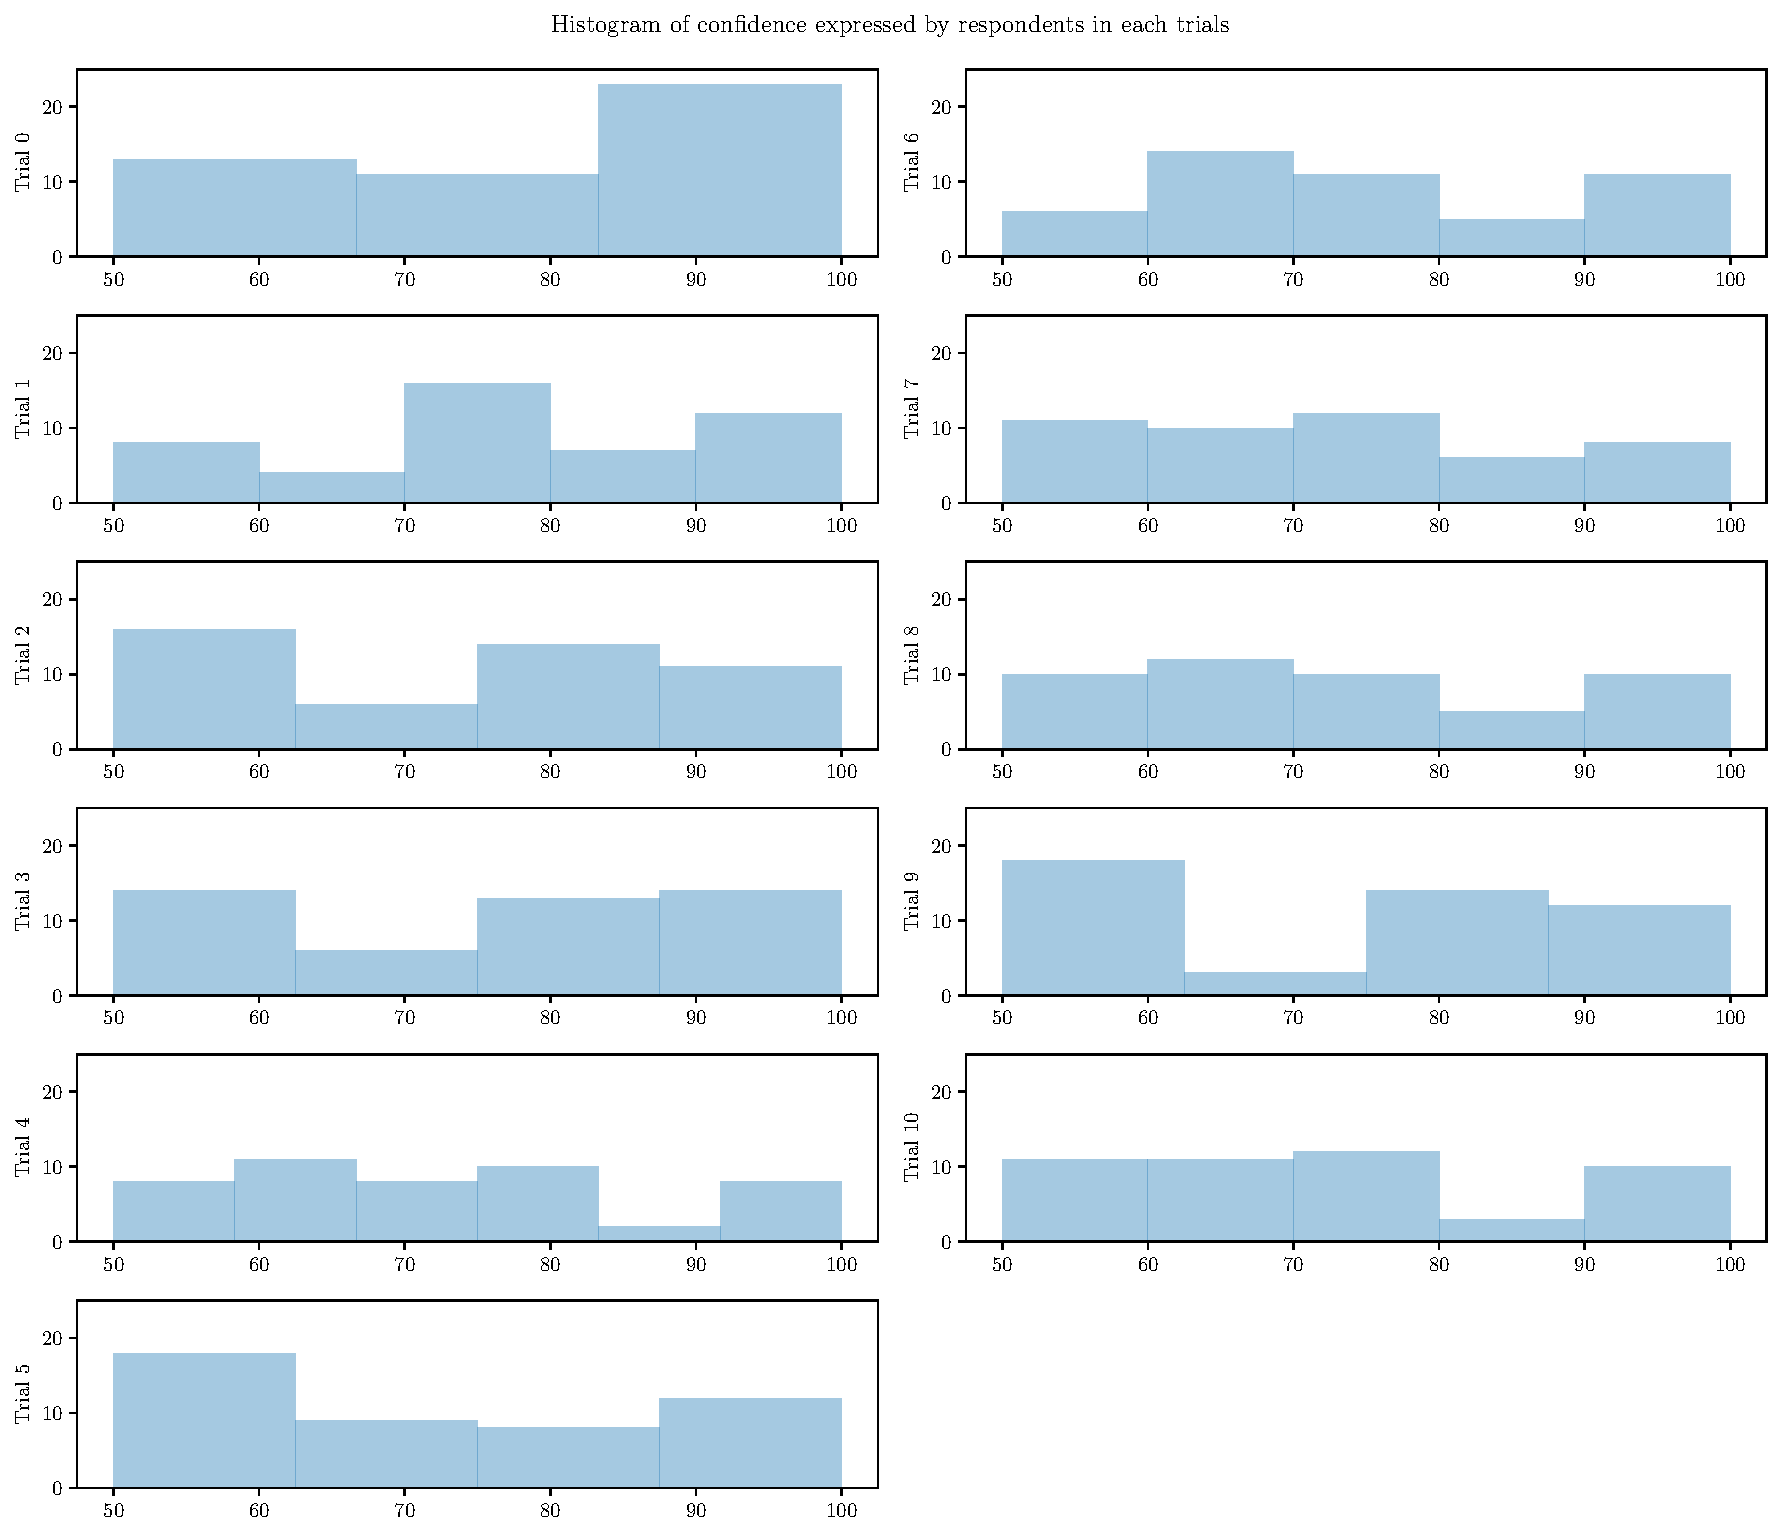
\includegraphics[width=\textwidth, center]{exp1_conf.pdf}
    \caption{Histogram of confidences in the experiment. Respondents report a wide range of confidence in most questions.}
    \label{fig:conf_hist}
\end{figure}
\end{minipage}
\end{center}


\newpage
\vspace*{-10mm}
\subsection{Estimation Scores}
We ask the respondents to give us an estimation of others' responses to the first question. Specifically, we ask them what percentage of the respondents would vote that the news piece is 'Real'.

For the Surprisingly Popular (SP) voting scheme, we need to compare the average estimation for the each of two answers to their actual votes. Whichever has a higher share of the votes than was estimated (on average), is the surprisingly popular scheme.

Figure \ref{fig:exp1_estim_trial0} shows the histogram  of estimations, divided based on the actual vote of participants into two partitions. The top panel shows the distribution of estimations made by those who voted 'Real' and the bottom panel shows the estimations of those who voted 'Fake.'

\begin{figure}[H]
    \centering
    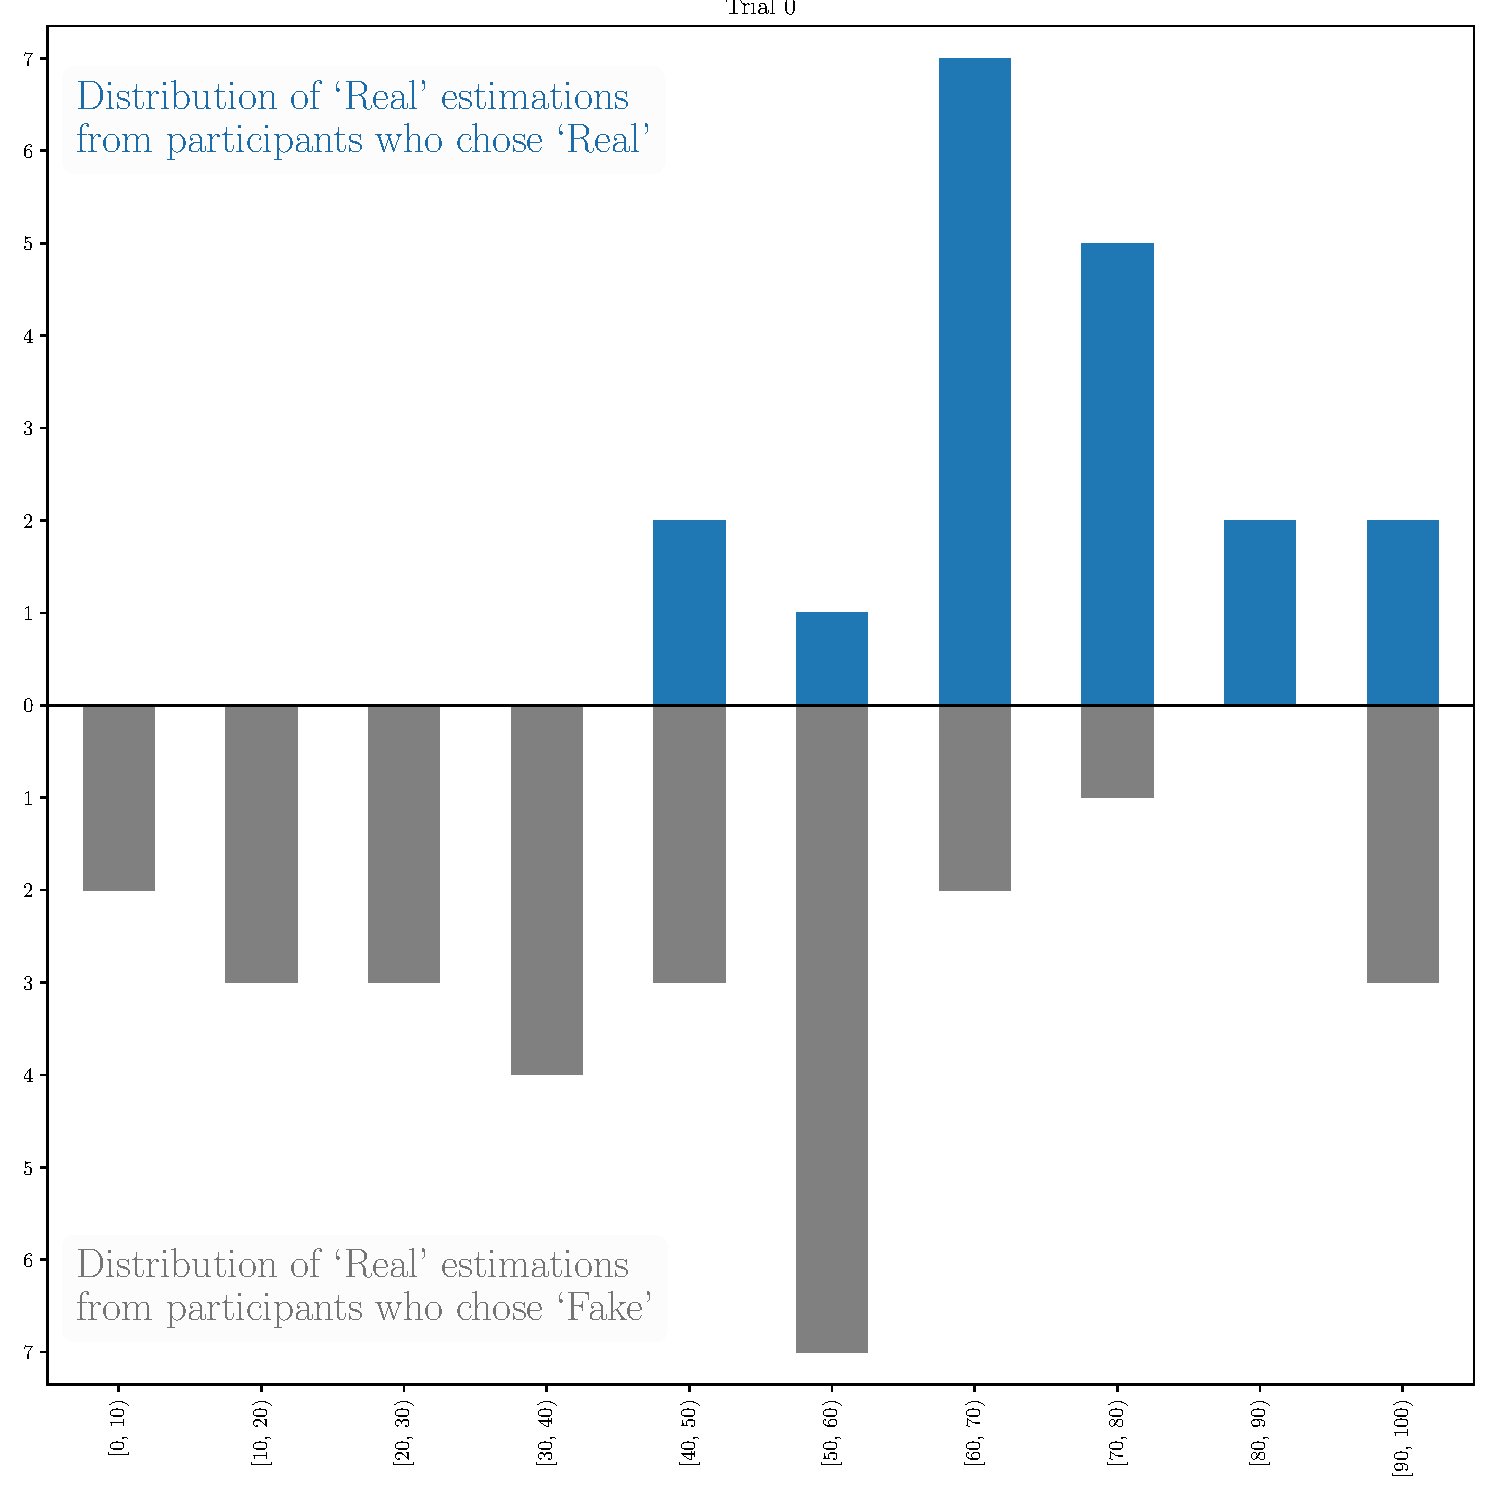
\includegraphics[width=\textwidth]{exp1_estim_trial0.pdf}
    \caption{Estimation histogram for Trial 0. The histograms has been divided into two partitions, depending on the actual vote of participants. Plot idea is credited to \cite{lee:NFL}.}
    \label{fig:exp1_estim_trial0}
\end{figure}

\subsection{Surprisingly Popular and Estimation Scores}
\label{sec:SP_estim_scores}
The intuition behind the SP voting mechanism is that either the `experts' (those who know the true answer to the 'real'/'fake' question) are in the majority, or if they are a minority, they know it themselves --- in the sense that they estimate that a majority of the population would choose the opposite of what they have chosen.

If neither of these conditions are met, the mechanism fails to detect the correct answer. The SP tries to assign as much weight as possible to the \emph{experts} in the population, even when they are in a minority. As such, the failure of SP signals the absence of expert opinion in the voting population. 

Figure \ref{fig:exp1_estim_all} shows histograms for all trials. SP fails in trials 0, 1, 3, 5 and 8. In Trial 0, the `experts' are in minority but they are seemingly unaware of this, since they still estimate that a majority will favor their position. Similarly in Trial 1, the experts (those who have chosen 'fake') estimate that most of the population would also think that the news is fake. The analysis for trials 5 and 8 are similar. 

In Trial 3, however, the experts seem to be in a majority, but their majority is not strong enough to compensate for the fact they too are over-estimating the population. However the difference is very small and with some minor filtering of the noisy data the decision can be corrected (see Section \ref{sec:sp_diag}).

\begin{center}
\begin{figure}
\hspace*{-3cm}
\begin{minipage}{1.5\linewidth}
    \centering
    \centerline{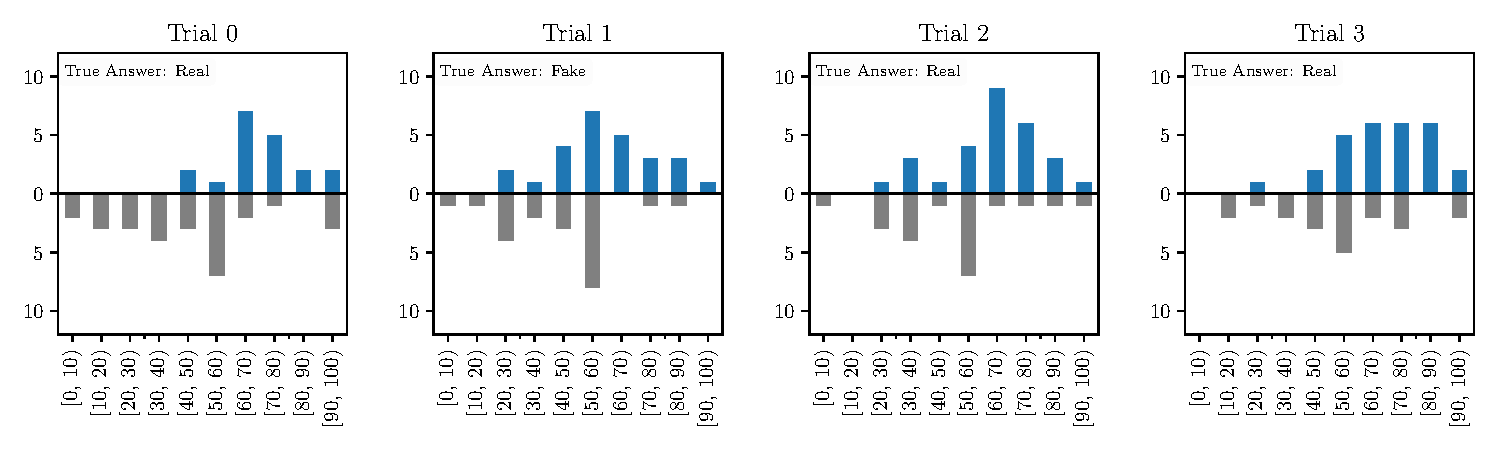
\includegraphics[width=\textwidth]{exp1_estim_0-3.pdf}}
    \centerline{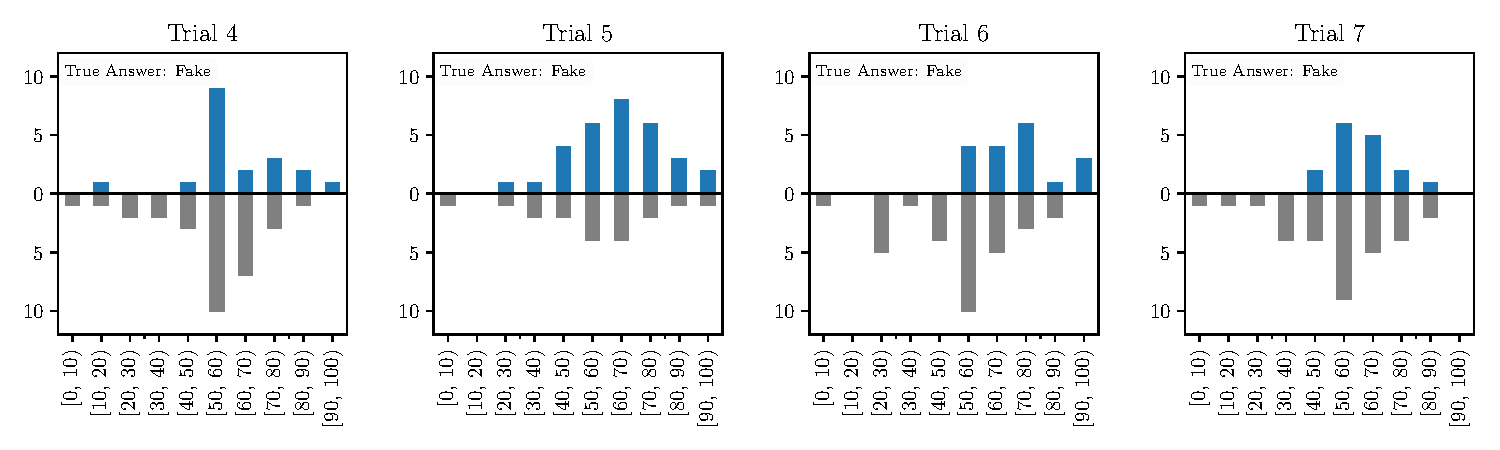
\includegraphics[width=\textwidth]{exp1_estim_4-7.pdf}}
    \centerline{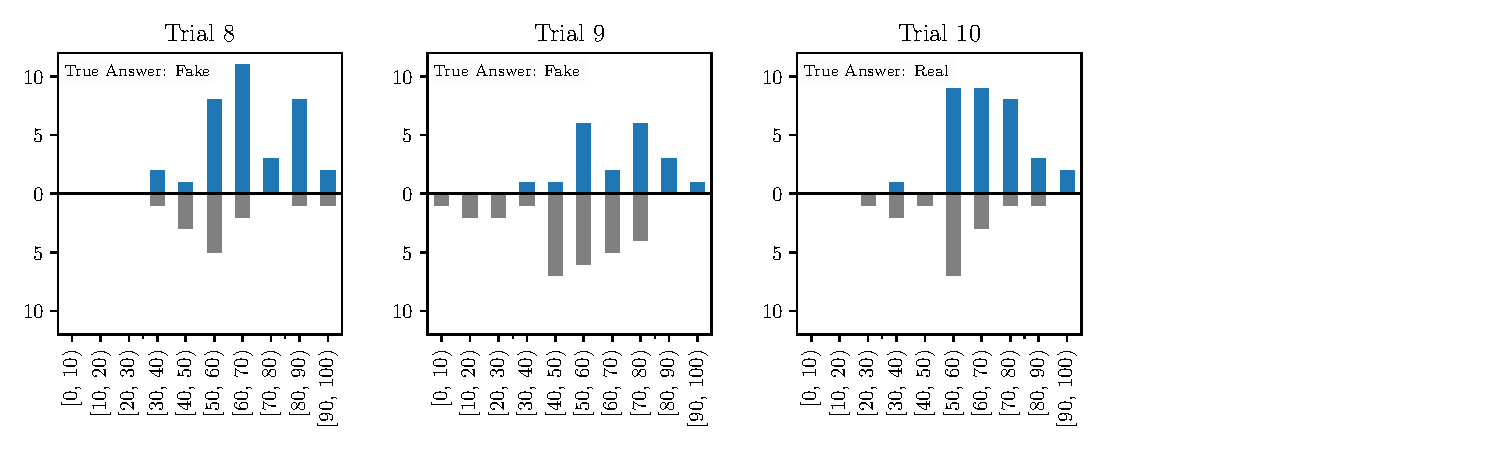
\includegraphics[width=\textwidth]{exp1_estim_8-10.pdf}}
    \caption{Estimation histograms for all trials. For the SP mechanism to work, `those who know' (who choose the right answer) should either be in the majority themselves or else estimate that `those who don't know are in the majority'. Without any filtering of the data, SP fails in trials 0, 1, 3, 5 and 8 because neither of these conditions hold. The data is too noisy, as respondents have not taken the time to assess others' potential response.}
    \label{fig:exp1_estim_all}
\end{minipage}
\end{figure}
\end{center}

\section{Timing Analysis}
We collected UNIX time-stamps from respondents' interactions with the questionnaire. We collected time-stamps at the start of each trial and at the times the respondent clicked to answer every question (see, for example, Figure \ref{fig:sample_question}). 

Using these statistics, we calculated the reading time, time spent answering Question 1 ('Real'/'Fake'), Question 2 (Confidence in answer) and Question 3 (Estimation of others' answers to Question 1, as well as the time spent to answer the validation question.

These statistics not only help us understand the behavior of the users, but also give us simple quality control measures. For example, if a user spends very little time answering the estimation question --- which is central to the SP algorithm --- then he or she can be removed from the estimation pool of SP, for that particular question. In Section \ref{sec:sp_diag} we will use this technique to investigate some of the problematic trials we observed in Figure \ref{fig:exp1_estim_all}.

\begin{figure}[H]
\hspace*{-3cm}
\begin{minipage}{1.5\linewidth}
\subsection{Reading Time}
    \centering
    \centerline{
    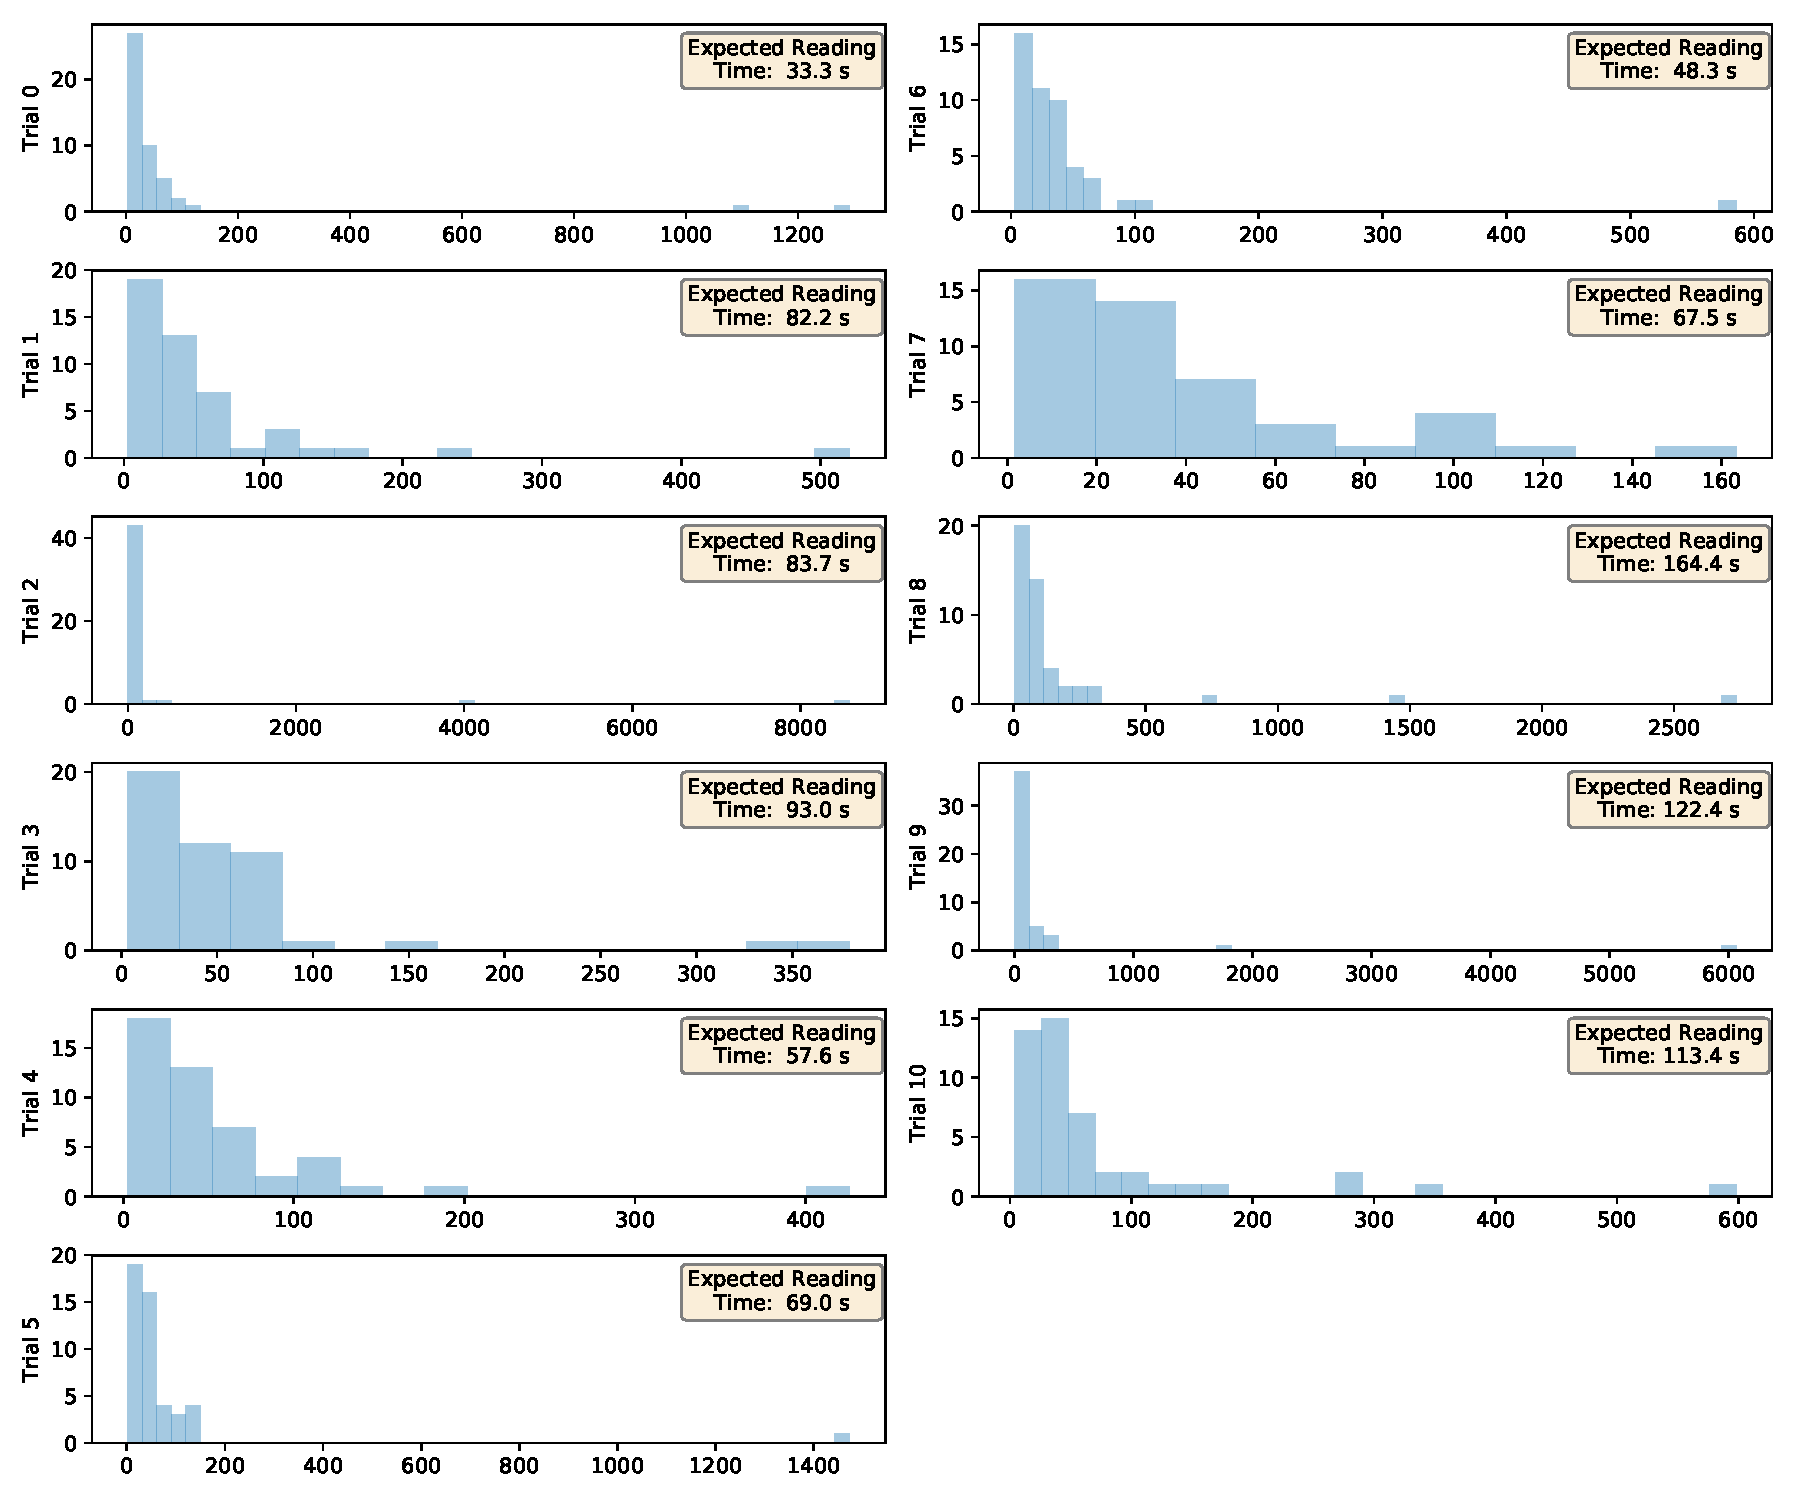
\includegraphics[width=\textwidth]{exp1_stats_reading.pdf}}
    \caption{Reading Time Statistics. The expected reading time is calculated based on word count of each news article, assuming an average reading speed of 200 words per minute.}
    \label{fig:exp1_stats_reading}
\end{minipage}
\end{figure}

\begin{figure}[H]
\hspace*{-3cm}
\begin{minipage}{1.5\linewidth}
\subsection{'Real'/ 'Fake' Time}
    \centering
    \centerline{
    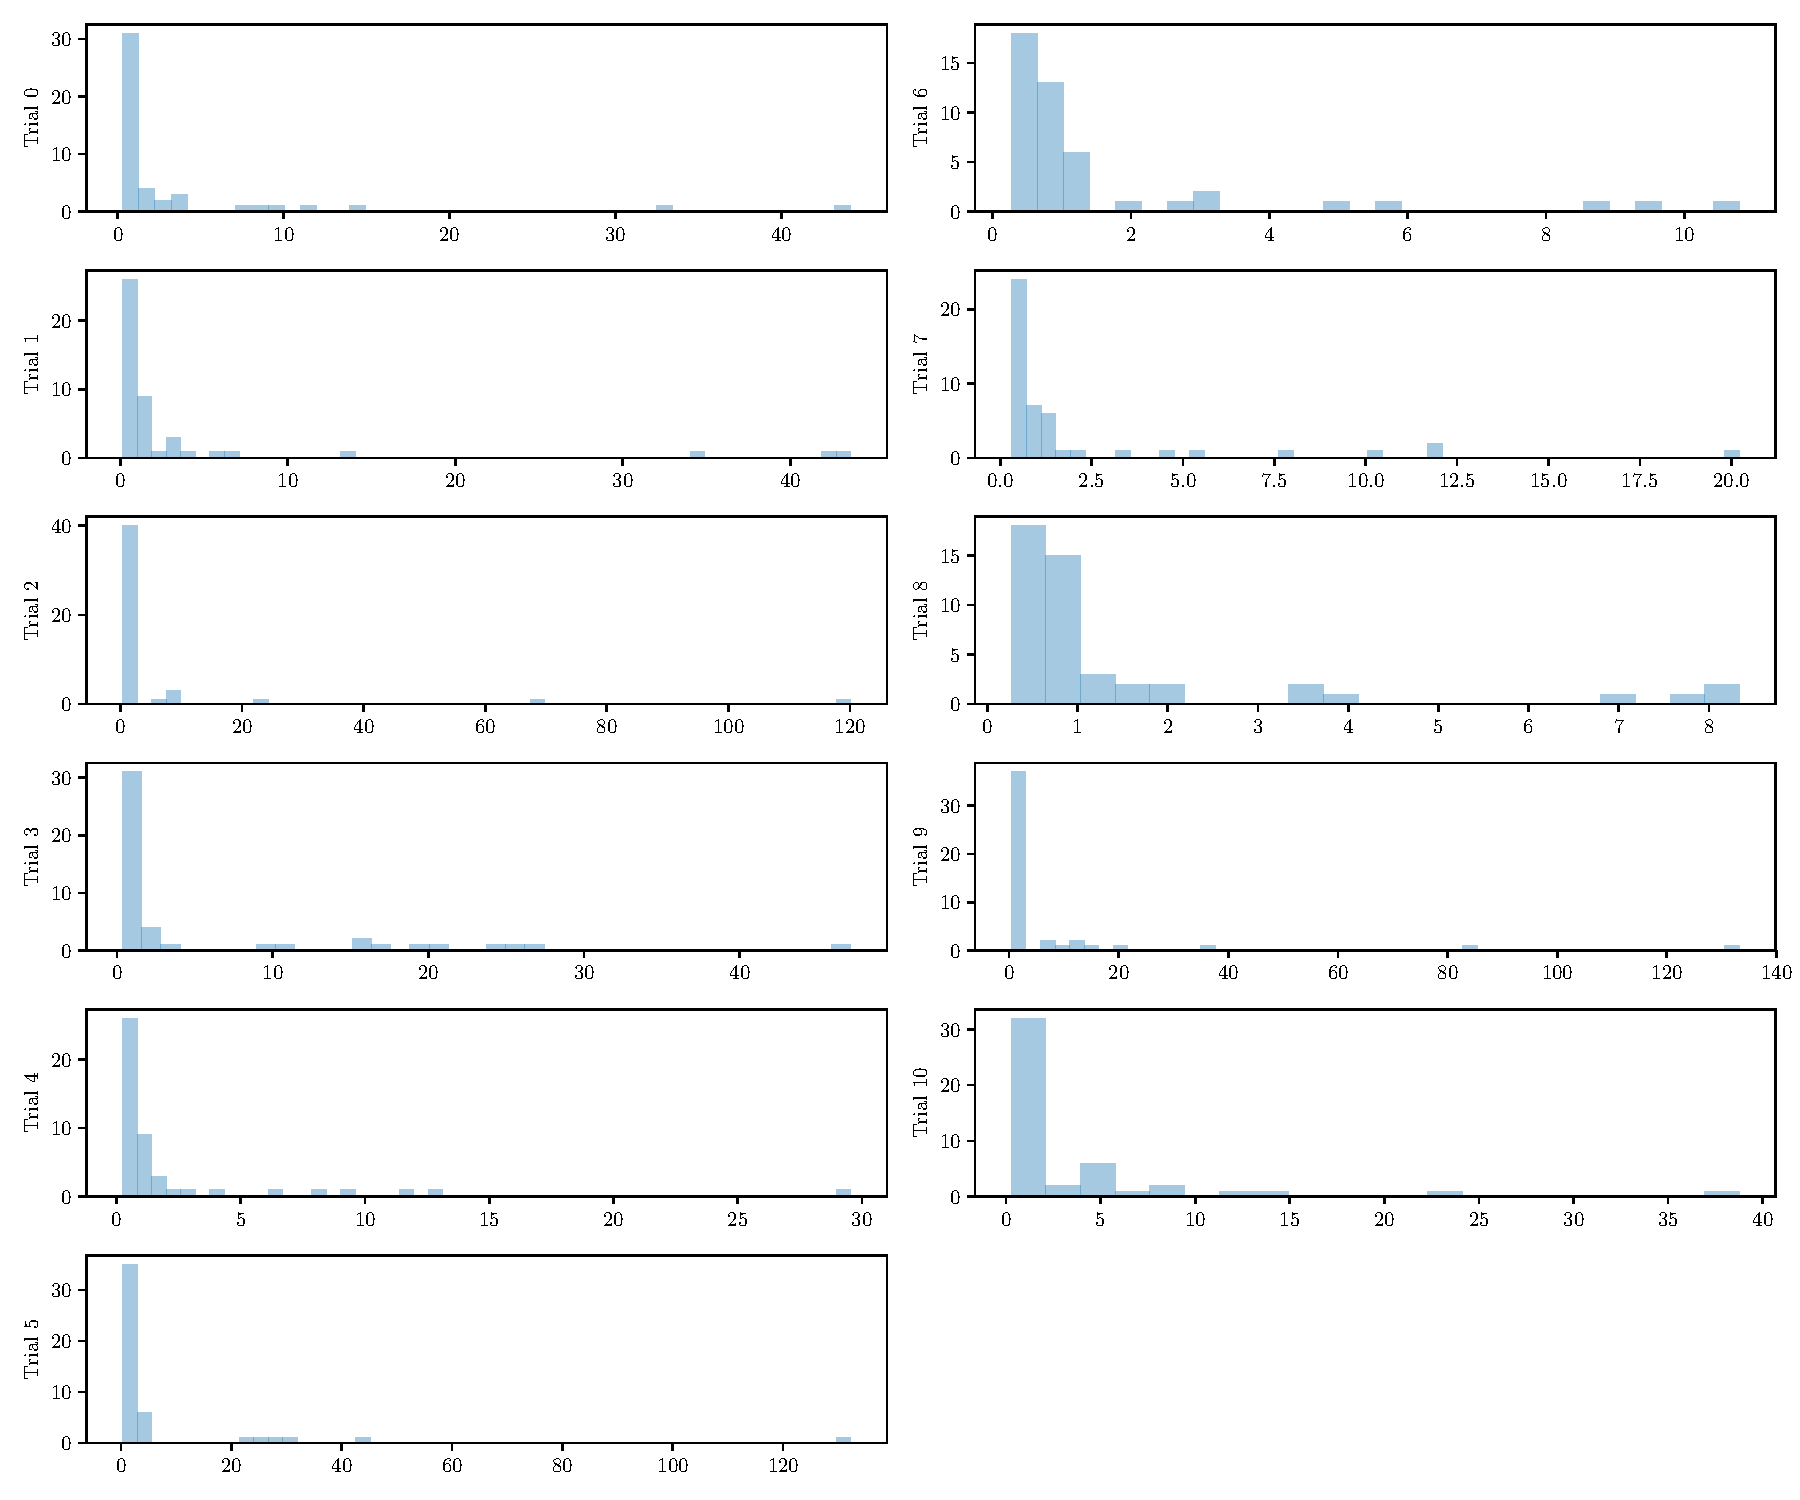
\includegraphics[width=\textwidth]{exp1_stats_real_fake.pdf}}
    \caption{Real/Fake Time Statistics}
    \label{fig:exp1_stats_real_fake}
\end{minipage}
\end{figure}

\begin{figure}[H]
\hspace*{-3cm}
\begin{minipage}{1.5\linewidth}
    \subsection{Confidence Time}
    \centering
    \centerline{
    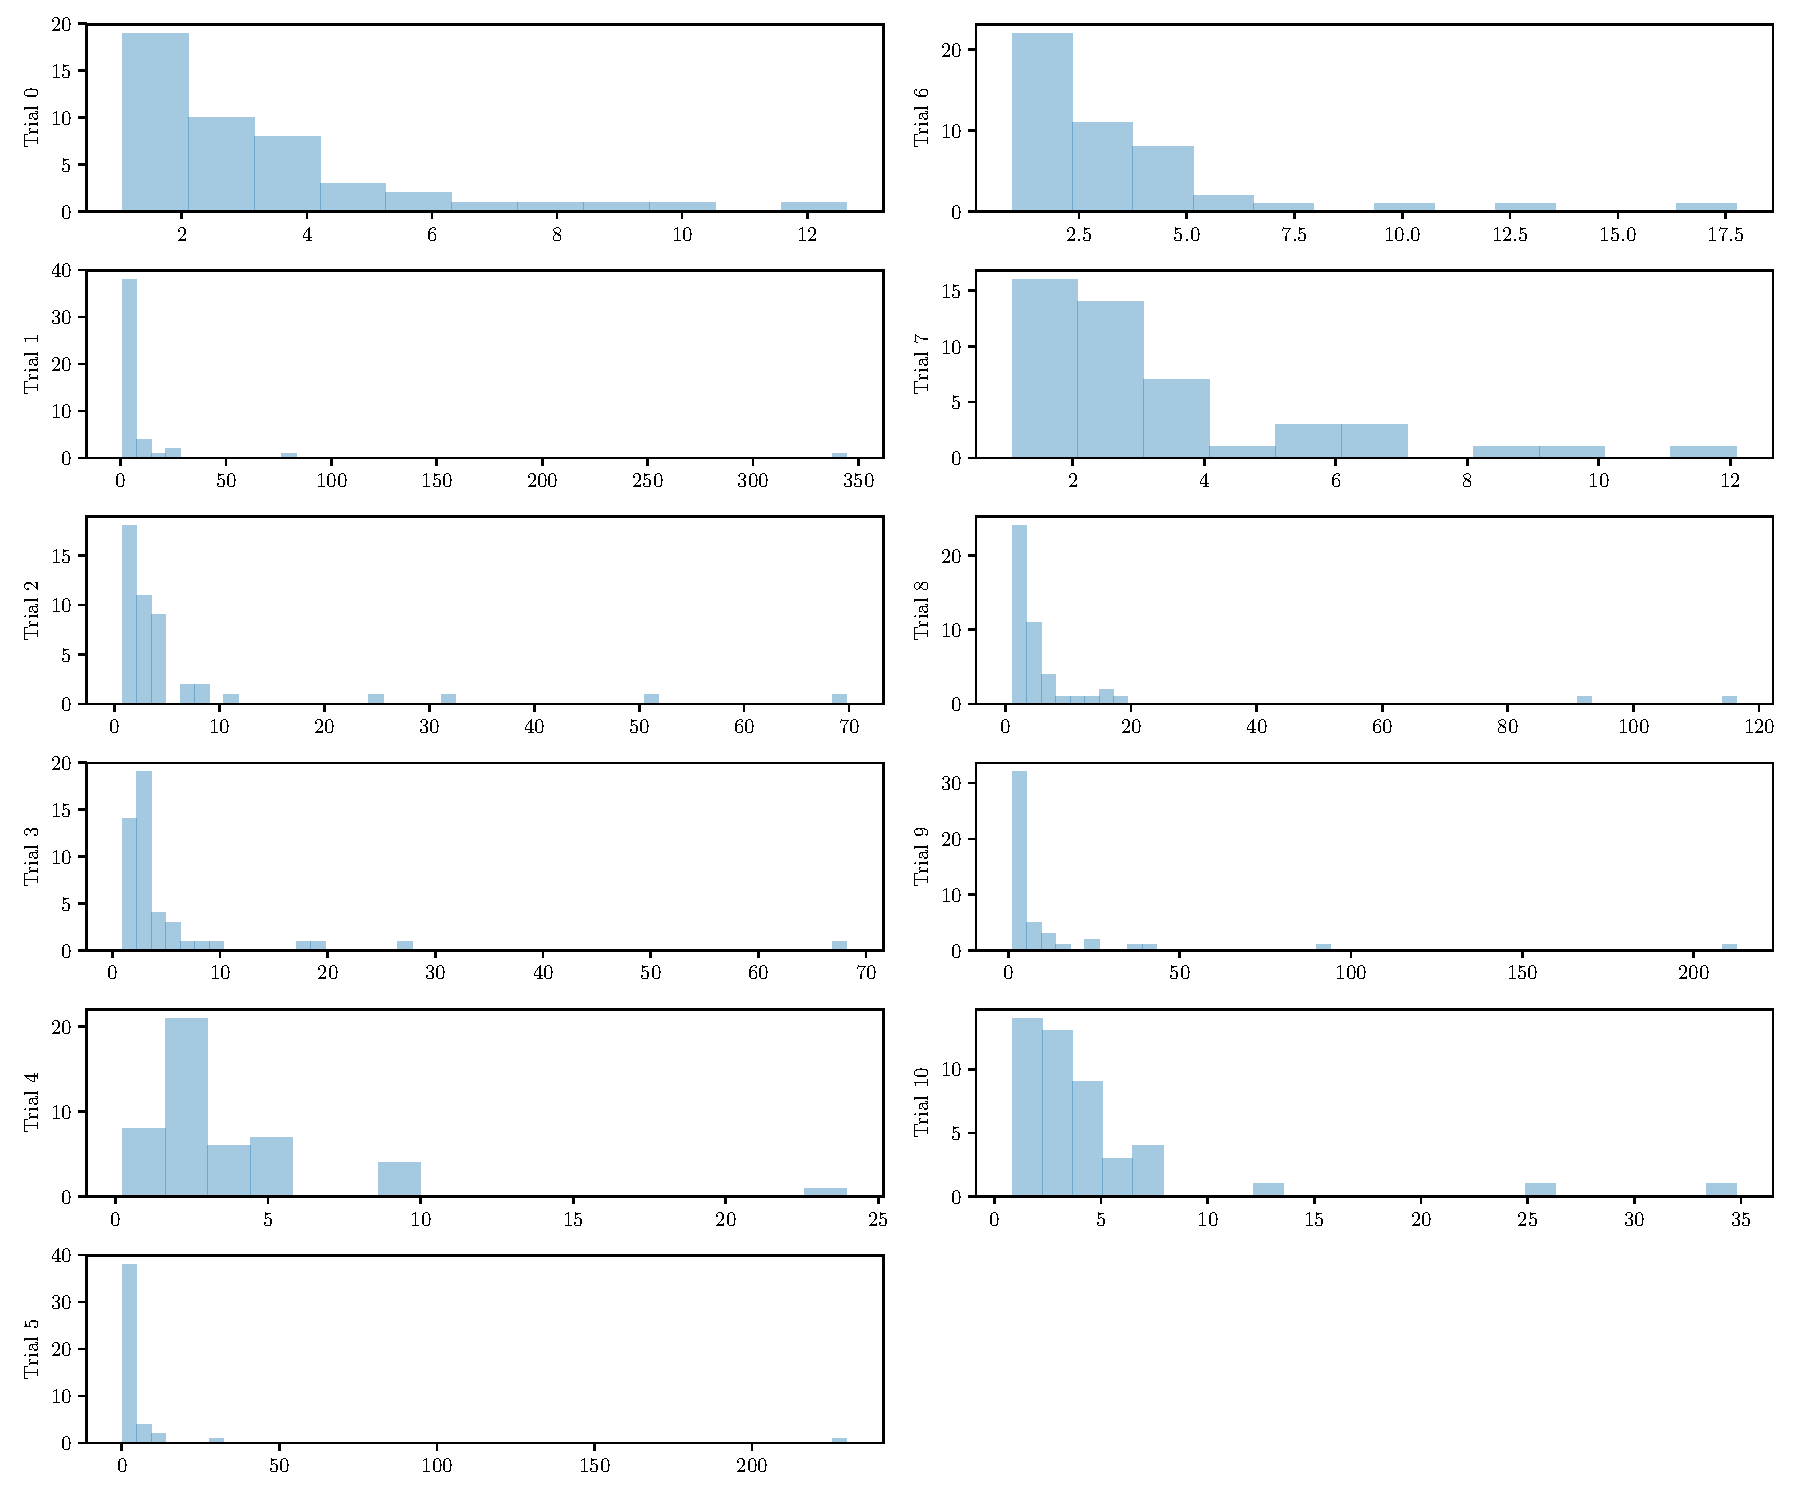
\includegraphics[width=\textwidth]{exp1_stats_conf.pdf}}
    \caption{Confidence Time Statistics}
    \label{fig:exp1_stats_conf}
\end{minipage}
\end{figure}

\begin{figure}[H]
\hspace*{-3cm}
\begin{minipage}{1.5\linewidth}
\subsection{Estimation Time}
    \centering
    \centerline{
    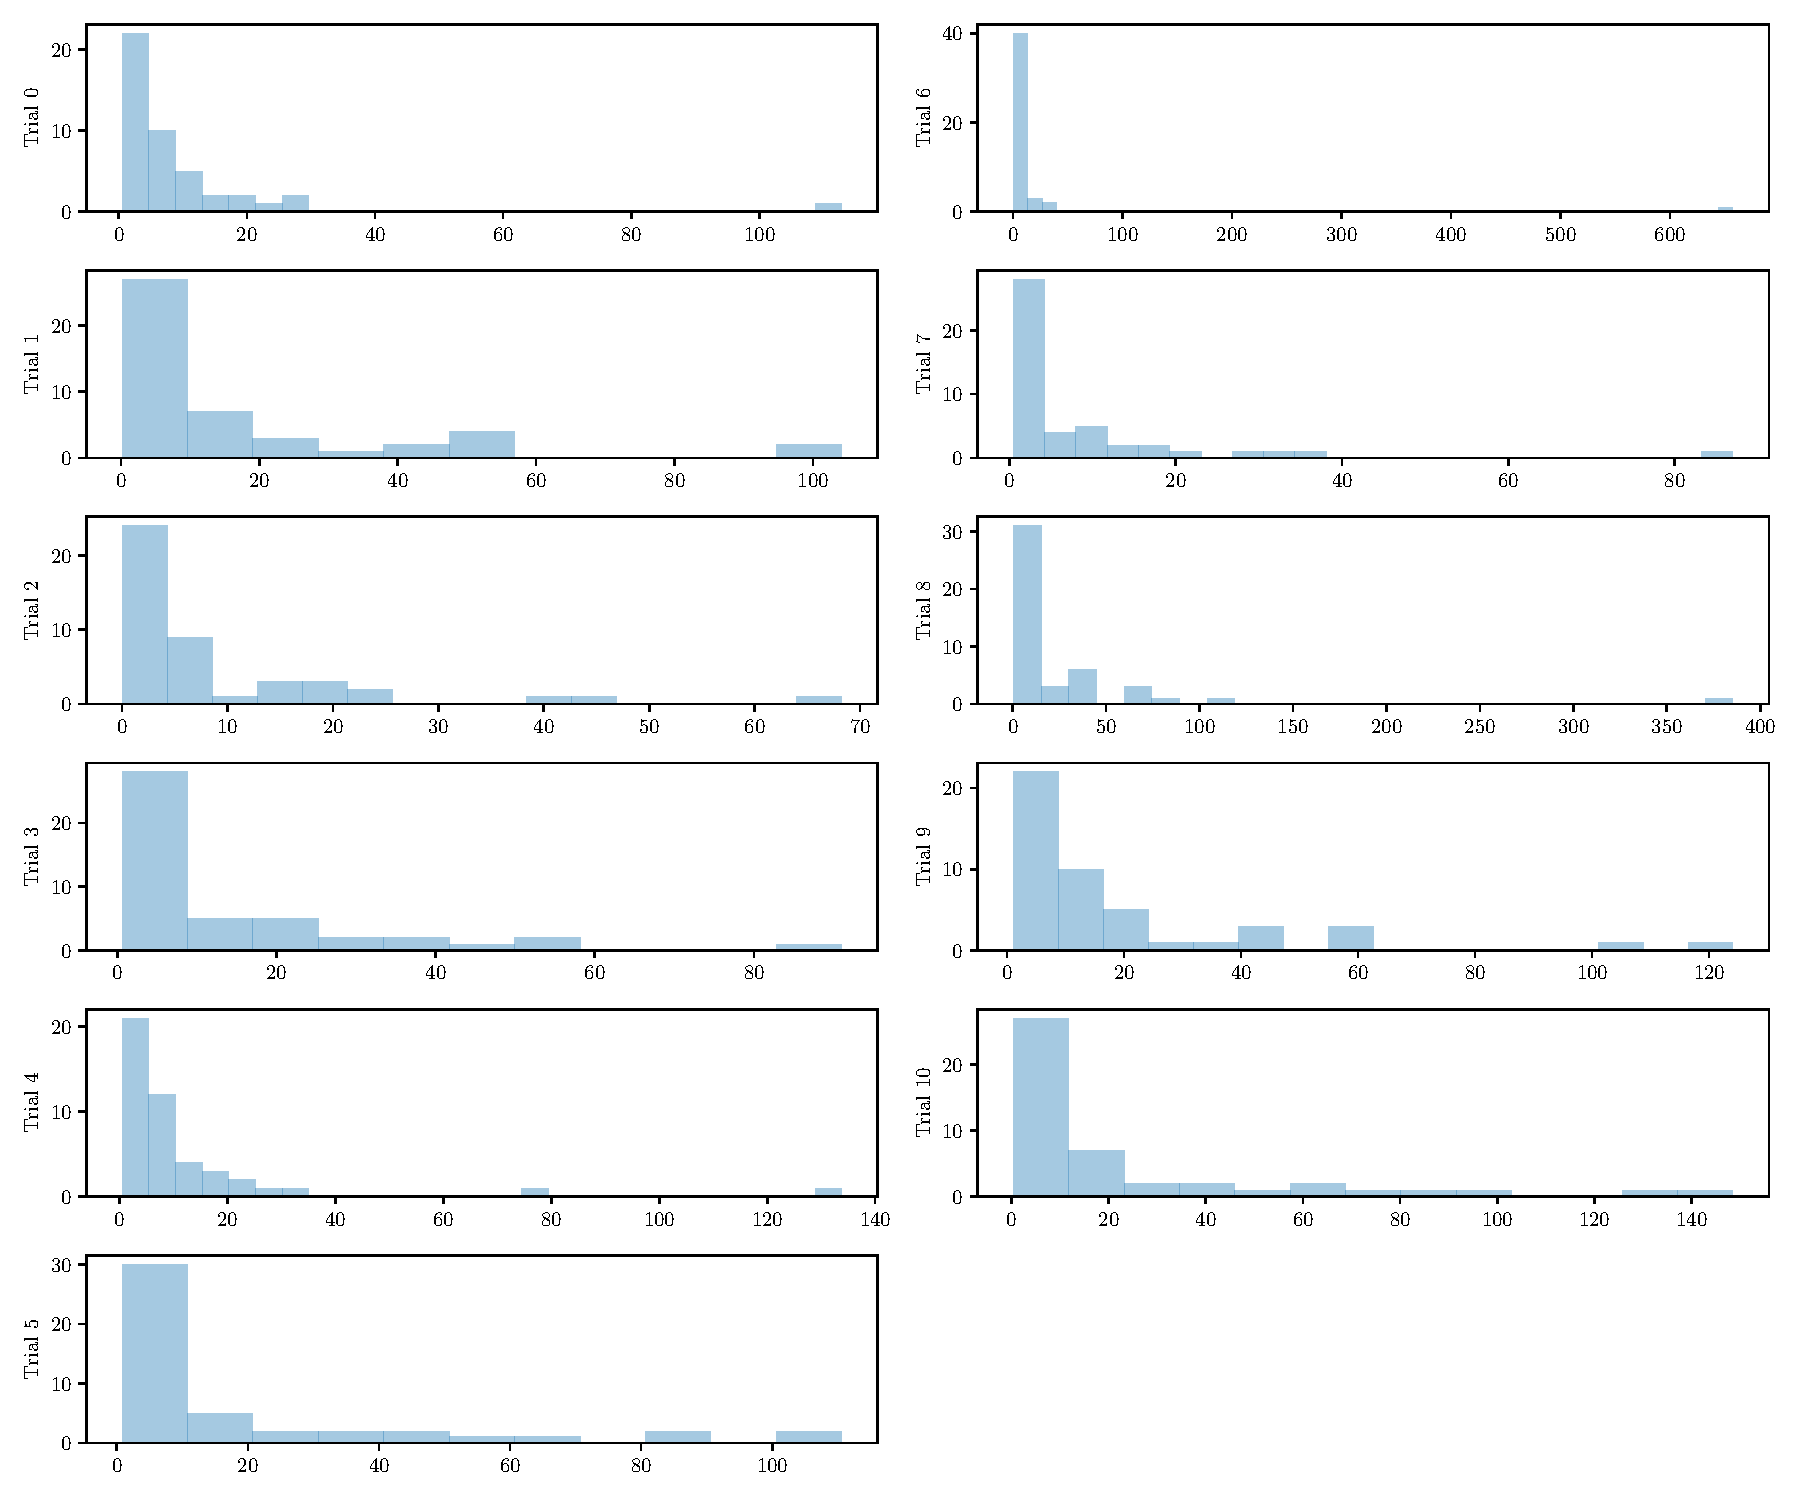
\includegraphics[width=\textwidth]{exp1_stats_estim.pdf}}
    \caption{Estimation Time Statistics}
    \label{fig:exp1_stats_estim}
\end{minipage}
\end{figure}


\begin{figure}[H]
\hspace*{-3cm}
\begin{minipage}{1.5\linewidth}
\subsection{Validation Time}
    \centering
    \centerline{
    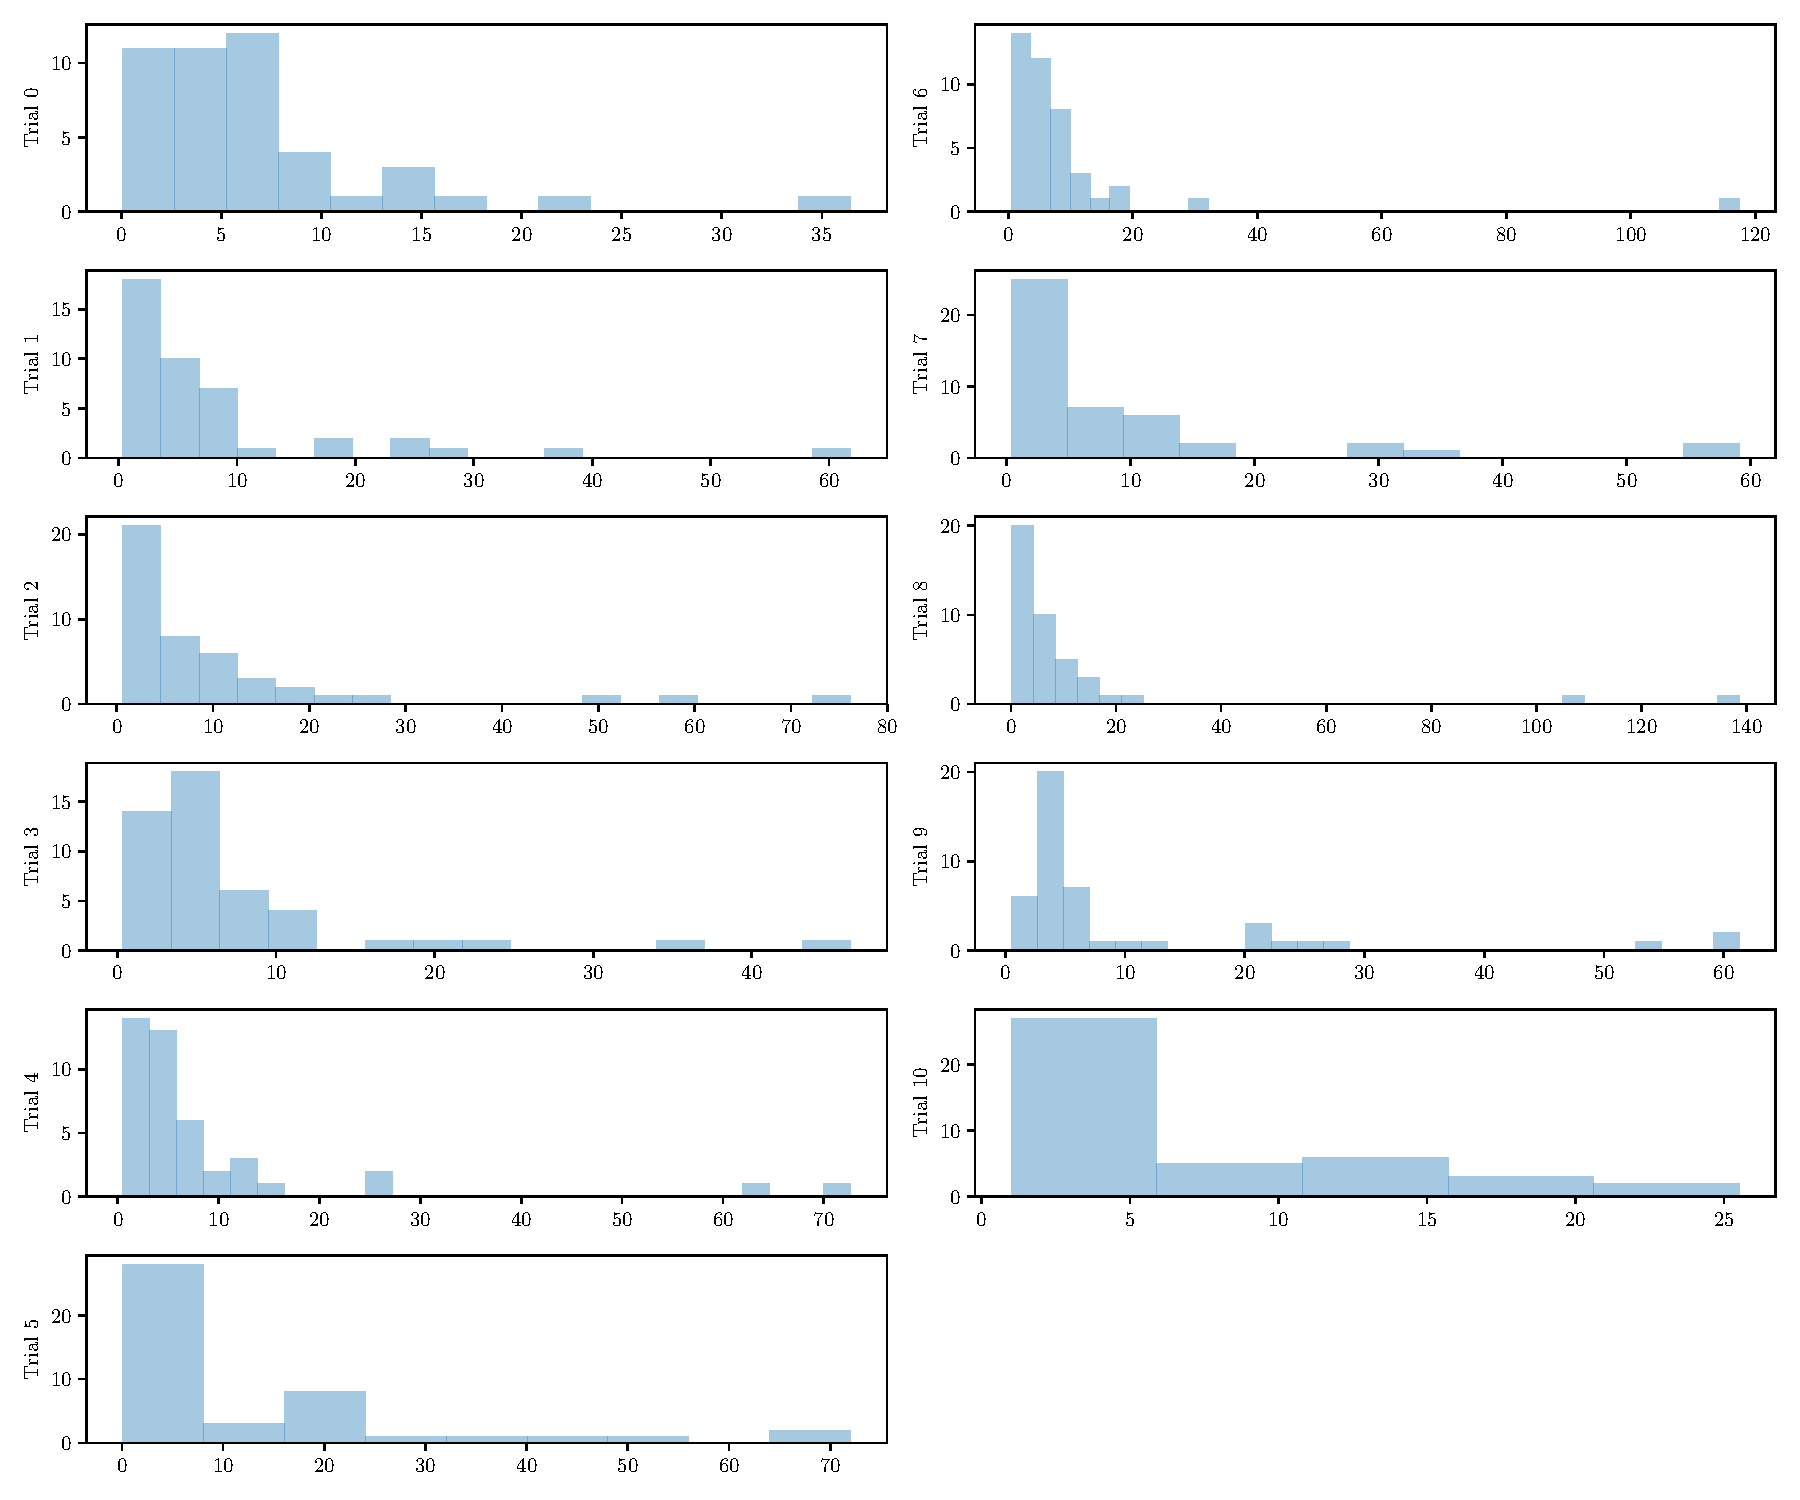
\includegraphics[width=\textwidth]{exp1_stats_valid.pdf}}
    \caption{Validation Time Statistics}
    \label{fig:exp1_stats_valid}
\end{minipage}
\end{figure}

\clearpage
\section{SP Diagnostics with Estimation Times}
\label{sec:sp_diag}
It is clear from Figure \ref{fig:exp1_stats_estim} that a majority of respondents  do not spend enough time answering the estimation question to the best of their knowledge. This causes major issues for voting schemes that use these measures. In this section, we propose filtering the candidate pool based on estimation time. Of course, this is not always possible. Excessive filtering can create degenerate cases where only a couple of samples remain. However, depending on the quantity and quality of the unfiltered data, this could prove essential for practical use of SP and other voting schemes.

\subsection{Case study: Trial 3}
As we also mentioned in Section \ref{sec:SP_estim_scores}, Trial 3 is a particular case, where although the experts are in majority, their majority is not strong enough to counter-act their poor estimation. The actual estimation difference is actually very small, only 1.96\%:

\begin{verbatim}
Trial 3
Answered Real: 57.45%
Answered Fake: 42.55%
Estimated Real: 59.40%
Estimated Fake: 40.60%
Difference(Real): -1.96%
Difference(Fake): 1.96%
SP Answer is: 'Fake'
True answer is: 'Real'
\end{verbatim}

This shows that filtering some of the noisy data using the estimation time threshold can tip the scale. Indeed, with only a 3 second threshold (meaning that only workers who spend at least 3 seconds contemplating the estimation question should be allowed in the estimation count), the SP decision changes:

\begin{verbatim}
  ==  Using filtering on "estimation" with threshold=5 seconds
Trial 3
Answered Real: 57.45%
Answered Fake: 42.55%
Estimated Real: 56.93%
Estimated Fake: 43.07%
Difference(Real): 0.52%
Difference(Fake): -0.52%
SP Answer is: 'Real'
True answer is: 'Real'  
\end{verbatim}

However the margin is very small, increasing the threshold can give us a more robust margin:

\begin{verbatim}
==  Using filtering on "estimation" with threshold=20 seconds
Trial 3
Answered Real: 57.45%
Answered Fake: 42.55%
Estimated Real: 47.22%
Estimated Fake: 52.78%
Difference(Real): 10.22%
Difference(Fake): -10.22%
SP Answer is: 'Real'
True answer is: 'Real'
\end{verbatim}


\section{Comparison with the baselines}
\label{sec:baseline_comparison}
\subsection{Baselines}
The main baseline is the majority vote. We also calculated a majority vote weighted with expressed confidences, but as it turns out the outcome of the vote did not change. We had hinted at this, when we observe the non-informativeness of the confidence signal in Section \ref{sec:conf}. Another baseline baseline we tried was filtering out respondents with accuracy smaller than 50\% and keeping the ``best respondents.''

\subsection{Results}
In the table below, CWMV stands for Confidence-Weighted Majority Vote, MV for Majority Vote, and `best' to filtering for the best (most accurate) respondents.

\begin{table}[H]
\footnotesize
\centerline{\begin{tabular}{lrrrrrrr}
\toprule
Trial &  CWMV (all) &  CWMV (best) &  MV (all) &  MV (best) &  SP (all) &  SP (best) &  Truth \\
\midrule
0  &        -1 &         -1 &      -1 &       -1 &      -1 &       -1 &          1 \\
1  &         1 &         -1 &       1 &       -1 &       1 &        1 &         -1 \\
2  &         1 &          1 &       1 &        1 &       1 &        1 &          1 \\
3  &         1 &          1 &       1 &        1 &      -1 &        1 &          1 \\
4  &        -1 &         -1 &      -1 &       -1 &      -1 &       -1 &         -1 \\
5  &         1 &          1 &       1 &        1 &       1 &        1 &         -1 \\
6  &        -1 &         -1 &      -1 &       -1 &      -1 &       -1 &         -1 \\
7  &        -1 &         -1 &      -1 &       -1 &      -1 &       -1 &         -1 \\
8  &         1 &          1 &       1 &        1 &       1 &        1 &         -1 \\
9  &        -1 &         -1 &      -1 &       -1 &      -1 &       -1 &         -1 \\
10 &         1 &          1 &       1 &        1 &       1 &        1 &          1 \\
\bottomrule
\end{tabular}}
\caption{Comparison of the results with \textbf{no filtering on estimation time.} 1 stands for 'Real' and -1 stands for 'Fake'. The mean results are SP~(all):~54.55\%, MV (all): 63.64\%, CWMV~(all):~63.64\%. Also for the best respondents: SP (best): 63.64\%, MV (best): 72.73\%, CWMV~(best): 72.73\%}
\label{tab:results_no_filtering}
\end{table}






\subsection{Cohen's Kappa} 
Cohen's Kappa is a score that expresses the level of agreement between two annotators on a classification problem. Here we use it as a measure of agreement between the outcome of each voting mechanism and the ground truth.
It is defined as
\begin{equation}
    \kappa = (p_o - p_e) / (1 - p_e)
\end{equation}

where $p_o$ is the empirical probability of agreement on the label assigned to any sample (the observed agreement ratio), and $p_e$ is the expected agreement when both annotators assign labels randomly. $p_e$ is estimated using a per-annotator empirical prior over the class labels.\cite{cohen:kappa}

Figure \ref{fig:exp1_cohen_kappa} shows the Cohen's kappa for different voting schemes. The last scheme is the Surprisingly Popular scheme with a threshold on estimation time. We observe that after filtering all participants who took less than 48 seconds to answer the estimation question, the SP beats the rest of the voting mechanisms.


\newpage
\thispagestyle{empty}
\begin{center}
\begin{figure}[H]
\vspace*{-3.2cm}
\hspace*{-3cm}
\begin{minipage}{1.43\linewidth}
    \centering
    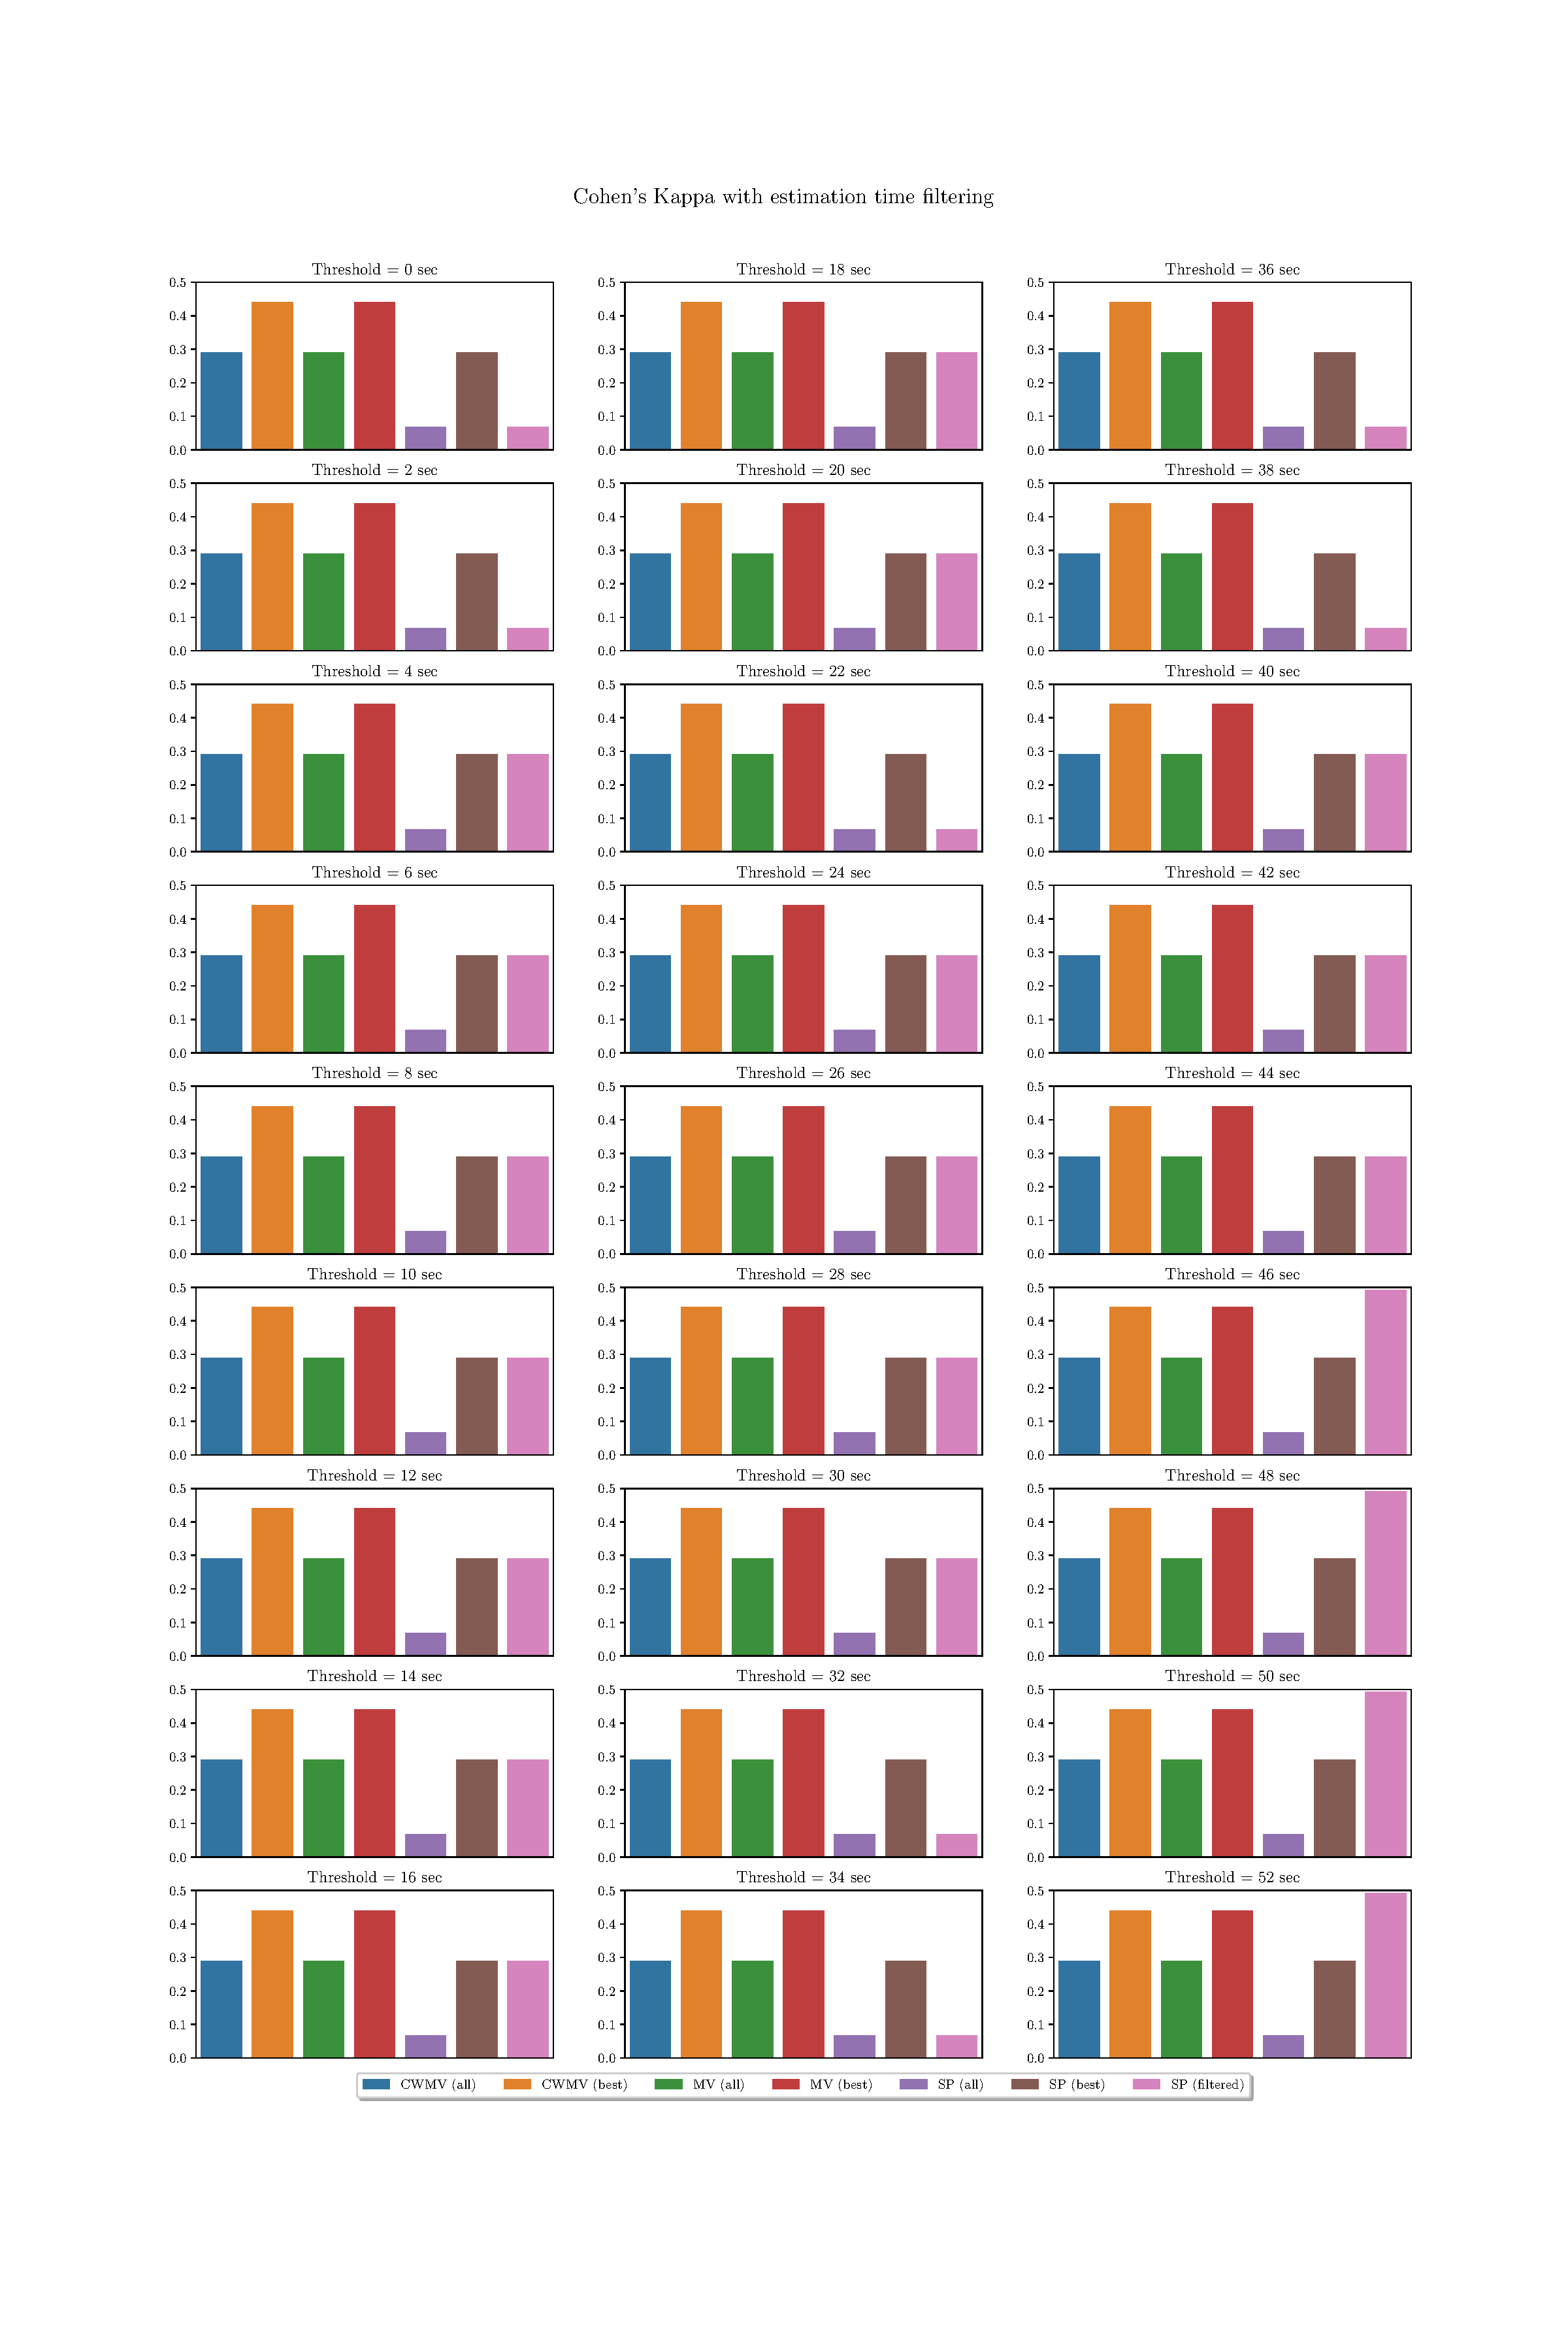
\includegraphics[width=\textwidth]{exp1_cohens_filtering.pdf}
    \caption{Cohen's kappa.}
    \label{fig:exp1_cohen_kappa}
\end{minipage}
\end{figure}
\end{center}

\printbibliography

\end{document}
